% !TeX TS-program = xelatex

\documentclass[11pt, a4paper]{report}

% Dokumentum adatok
% =================
\author{}
\title{Műszaki hőtan feladatgyűjtemény}

% A közös fájlok beszúrása
% ========================
\newcommand*{\JakiFolder}{./JAKI}%

% A közös fájlok a JAKI tárolóban vannak, amit az MHFGY-vel 
% közös mappába kell letölteni (clone/pull).

% A "book" dokumentumosztály fölösleges oldalakat szúr be a címoldal
% és a tartalomjegyzék után.

\usepackage[utf8]{inputenc}
\usepackage[magyar]{babel}

% XeLaTeX ékezetes betűk
\usepackage{fontspec}

% A margók beállítása, később a 
%	\newgeometry{left=3cm,bottom=0.1cm}
% és a 
%	\restoregeometry
% parancsokkal egyedileg módosíthatók a margók
\usepackage[left=2cm, right=2cm, top=2cm, bottom=2cm]{geometry}

\usepackage{amsmath}
\usepackage{amssymb}

% A dupla betűk betűtípusának beállítása
\AtBeginDocument{
	\DeclareSymbolFont{AMSb}{U}{msb}{m}{n}
	\DeclareSymbolFontAlphabet{\mathbb}{AMSb}
}

% A régi német betűtípusok támogatása (fraktúra, Schwabacher, gót)
% A gót betűtípus nem működik
% Az ékezetes betűk csak a Table 18: Text-mode Accents táblázat szerint működnek
\usepackage{yfonts}

% Tabu hiba kezelés
\usepackage{booktabs}% http://ctan.org/pkg/booktabs
\newcommand\tabitem{\makebox[1em][r]{\textbullet~}}
\usepackage{tabto}
\usepackage{tabu}

% Bekeretezett részek
\usepackage[framemethod=tikz]{mdframed}
% Megjegyzés
\newcommand{\comment}[2][black!10]{%
\begin{mdframed}[hidealllines=true, backgroundcolor=#1, innerleftmargin=3pt, innerrightmargin=3pt, leftmargin=-3pt, rightmargin=-3pt]
Megjegyzés: #2
\end{mdframed}
}

%\usepackage{titlesec}

\pagestyle{plain}

\usepackage{float}
\usepackage{xifthen}

% Tizedesvessző
\usepackage{icomma}

% Függelék

\usepackage[toc,titletoc,page]{appendix}
\renewcommand{\appendixtocname}{Függelékek}
\renewcommand{\appendixpagename}{Függelékek}


%\fontspec{Times New Roman}
%\setmonofont{Consolas}
%\setmainfont{Calibri}

\usepackage{commath}
% A \Dif esetén a hatványkitevők rálógnak a D-re.
% A deriváltakban a d után sok az üres hely.

% This package will provide a complete implementation of 
% unicode maths for XELATEX and LuaLATEX.
% A Cambria Math támogatott.
% Javítja a vektor jelek elhelyezését a betűk felett.
% Az alsó és felső indexek betűtípusait módosítja, és szélesebbek a betűk.
\usepackage[math-style=TeX]{unicode-math}
%\setmathfont{XITS Math} % Túl vastagok a betűk
%\setmathfont{Cambria Math}

\usepackage{siunitx}
\sisetup{
	per-mode = fraction,
	fraction-function = \dfrac,
	detect-family = true,
	output-decimal-marker = {,},
	space-before-unit = true,
	use-xspace = true,
	exponent-product = \cdot,
	sticky-per = true
}

\usepackage[makeroom]{cancel}

% Többrészes ábrák létrehozása, subfigure környezet
\usepackage[justification=centering]{caption}
\usepackage{subcaption}

% A Hyperref csomagot lehetőleg utolsóként kell betölteni.
\usepackage[colorlinks=false]{hyperref}

% A címsorok másolása a kereszthivatkozásokba
\usepackage{nameref}

% Bekarikázott számok
\usepackage{pifont}

% Kiemelés színnel
\usepackage{xcolor}

% Az oszlopvektorok és mátrixok jelölésére
\usepackage{accents}
\newcommand{\ubar}[1]{\underaccent{\bar}{#1}}

% Színes táblázat, a tabuhoz nem szükséges
%\usepackage{colortbl}

% Fekvő oldalak
% If you are using pdfLaTeX, you should use pdflscape instead. The pdflscape package adds PDF support to the landscape environment of package lscape, by setting the PDF/Rotate page attribute. Pages with this attribute will be displayed in landscape orientation by conforming PDF viewers:
\usepackage{pdflscape}

% Kiemelés
% Több sorba osztásnál %-ezni kell a sortöréseket
%\newcommand{\highlight}[2]{\colorbox{#1}{$\displaystyle#2$}}

% Függőleges távolságok
\newcommand{\reducedstrut}{\vrule width 0pt height 1.2\ht\strutbox depth 0.95\dp\strutbox\relax}
\newcommand{\highlight}[2]{%
  \begingroup
  \setlength{\fboxsep}{1pt}% Vízszintes távolság
  \colorbox{#1}{\reducedstrut$\displaystyle#2$\/}%
  \endgroup
}

% Sortáv módosítás
\usepackage{setspace}
%\singlespacing
%\onehalfspacing
%\doublespacing

% Felsorolások
\usepackage{enumitem}

% Megjegyzés létrehozás
%\newlist{notes}{enumerate}{1}
%\setlist[notes]{label=Megjegyzés: , leftmargin=*}

% Külső fájlok írása
% Elvileg szükségtelen
%\usepackage{filecontents}

% Forráskezelés
%When using babel or polyglossia with biblatex, loading csquotes is recommended to ensure that quoted texts are typeset according to the rules of your main language.
\usepackage{csquotes}
\usepackage[ 
	backend=biber, 
	url=false, 
	citestyle=numeric,%draft,
	bibstyle=numeric,%style=numeric,%authoryear,%numeric, 
	giveninits=true, 
	clearlang=true, 
	bibencoding=auto,
	sorting=none]{biblatex}
	
\makeatletter

\newrobustcmd*{\parentexttrack}[1]{%
  \begingroup
  \blx@blxinit
  \blx@setsfcodes
  \blx@bibopenparen#1\blx@bibcloseparen
  \endgroup}

\AtEveryCite{%
  \let\parentext=\parentexttrack%
  \let\bibopenparen=\bibopenbracket%
  \let\bibcloseparen=\bibclosebracket}

\makeatother


% Az egyenletek előtti és utáni térközök beállítása
% A TikZ blokkdiagamban a 3. szinttől lefele fölösleges bal margót hoz létre (???)
%
% => NE LEGYEN ÜRES SOR AZ EGYENLETEK ELŐTT!
%
%\makeatletter
%\g@addto@macro\normalsize{%
%	\setlength\abovedisplayskip{6pt}
%	\setlength\belowdisplayskip{12pt}
%	\setlength\abovedisplayshortskip{0pt}
%	\setlength\belowdisplayshortskip{12pt}
%}
%\makeatother

% Az árva- és özvegysorok büntetése (nem biztos, hogy nem lesznek...)
\widowpenalty10000
\clubpenalty10000


% SAJÁT PARANCSOK LÉTREHOZÁSA
% ===========================

\DeclareMathOperator{\tr}{tr}

% Gradiens, forráserősség, örvényerősség
\newcommand{\Grad}[1] {\mathrm{grad\,} #1}
\newcommand{\Div}[1] {\mathrm{div\,} #1}
\newcommand{\Rot}[1] {\mathrm{rot\,} #1}
\newcommand{\Diag}[1] {\mathrm{diag\,} #1}

% Függvények
\newcommand{\Det}[1] {\mathrm{det} #1}
\DeclareMathOperator{\tg}{tg}
\DeclareMathOperator{\sgn}{sgn}
\DeclareMathOperator{\arctg}{arctg}
\DeclareMathOperator{\arctgNN}{arctg2}

% Mátrix belső közei
\makeatletter
\renewcommand*\env@matrix[1][\arraystretch]{%
	\edef\arraystretch{#1}%
	\hskip -\arraycolsep
	\let\@ifnextchar\new@ifnextchar
	\array{*\c@MaxMatrixCols c}}
\makeatother

% Oszlopvektor, sorvektor és mátrix jelölések
\newcommand{\mat}[1] {\underline{\underline{#1}}\reducedstrut}
\newcommand{\cvec}[1] {\underline{#1}\reducedstrut}
%\def\rvec#1{\underline{#1}^{T}}
%\def\mat#1{\underline{\underline{#1}}}
%\def\mat3#1{\underline{\underline{\underline{#1}}}}

\newcommand{\vektor}[2][1]{\begin{bmatrix}[#1] #2 \end{bmatrix}}
\newcommand{\tmb}[2][2]{\begin{bmatrix}[#1] #2 \end{bmatrix}}
\newcommand{\vek}[4][1]{\begin{bmatrix}[#1] #2 \\ #3 \\ #4 \end{bmatrix}}
\newcommand{\mtrx}[1]{\begin{bmatrix}#1\end{bmatrix}}



% FÜGGELÉK TARTALOMJEGYZÉK
% Appendix csomag (appendix.sty)
%\newcommand{\@redotocentry@pp}[1]{%
%  \let\oldacl@pp=\addcontentsline
%  \def\addcontentsline##1##2##3{%
%    \def\@pptempa{##1}\def\@pptempb{toc}%
%    \ifx\@pptempa\@pptempb
%      \def\@pptempa{##2}\def\@pptempb{#1}%
%      \ifx\@pptempa\@pptempb
%\oldacl@pp{##1}{##2}{##3}%A kísérleti változat: \oldacl@pp{##1}{##2}{\appendixname\space [##1][##2][##3] (\@car \splitlist{##3}\@nil) (\@cdr \splitlist{##3}\@nil)}%
%      \else
%        \oldacl@pp{##1}{##2}{##3}%
%      \fi
%    \else
%      \oldacl@pp{##1}{##2}{##3}%
%    \fi}
%}


% VÁLTOZÓK
\makeatletter
\let\JakiTitle\@title
\let\JakiAuthor\@author
\makeatother

% OLDALSZÁMOZÁS
% Oldalszámozás váltás a kezdő, a fő és a befejező szakasz határán
% A "report" osztályban nincs, a "book" osztályból másolva...
%https://tex.stackexchange.com/questions/154646/is-there-an-easy-way-to-get-the-frontmatter-mainmatter-and-backmatter-in-a-l
\makeatletter
\newcommand\frontmatterreport{%
	\cleardoublepage
	%\@mainmatterfalse
	\pagenumbering{Roman}}

\newcommand\mainmatterreport{%
	\cleardoublepage
	%\@mainmattertrue
	\pagenumbering{arabic}}

\newcommand\backmatterreport{%
	\if@openright
		\cleardoublepage
	\else
		\clearpage
	\fi
	% \@mainmatterfalse
	}
\makeatother


% HYPERREF
\hypersetup{
	pdftitle={\JakiTitle}, 
	pdfauthor={\JakiAuthor}, 
	colorlinks = true,
	citecolor = orange,
	filecolor = red,
	linkcolor = blue,
	urlcolor = red
}


% Az átmérőjel alapvonalra emelése
%\makeatletter
%\let\olddiameter\diameter
%\renewcommand{\diameter}[0]{\raisebox{\depth}{\olddiameter}}
%\makeatother

				% Formázás, csomagok
% TikZ - Ábrázolás
% ================
\usepackage{tikz} 
\usepackage{tikz-3dplot}
\usetikzlibrary{arrows.meta, automata, bending, calc, decorations.markings, fit, graphs, intersections, patterns, positioning, scopes, shapes, shapes.geometric, shapes.multipart, trees}
% bending: a nyílfejek "elnyomják" az íveket, ez a könyvtár helyre teszi...

\usepackage{pgfplots}
\pgfplotsset{compat=1.10}
\usepgfplotslibrary{fillbetween}

% Szögek méretezése
% =================

\pgfkeys{/tikz/.cd, % to set the path
	xa/.initial=0, % initial value
	xa/.get=\xa, % to get the value from a macro
	xa/.store in=\xa, % to store the value into a macro
	xb/.initial=0,
	xb/.get=\xb,
	xb/.store in=\xb,
	ya/.initial=0,
	ya/.get=\ya,
	ya/.store in=\ya,
	yb/.initial=0,
	yb/.get=\yb,
	yb/.store in=\yb,
	ra/.initial=1.25 cm,
	ra/.get=\ra,
	ra/.store in=\ra,
	rb/.initial=1.5 cm,
	rb/.get=\rb,
	rb/.store in=\rb,
	rm/.initial=0.5cm,			% \pgfangle: sugár a méretvonal töréspontjáig
	rm/.get=\rm,
	rm/.store in=\rm,
	a/.initial=0,				% \pgfangle: szög (honnan); \pgflength: nyílfej van/nincs
	a/.get=\a,
	a/.store in=\a,
	b/.initial=45,				% \pgfangle: szög (hova); \pgflength: nyílfej van/nincs
	b/.get=\b,
	b/.store in=\b,
	lv/.initial=45,
	lv/.get=\lv,
	lv/.store in=\lv,
	lm/.initial=0.5,
	lm/.get=\lm,
	lm/.store in=\lm,
	alim/.initial=0,			% \pgflength: 0/[1] bal és jobb méretsegédvonal
	alim/.get=\alim,
	alim/.store in=\alim,
	blim/.initial=0,
	blim/.get=\blim,
	blim/.store in=\blim,
	ny/.initial=1,				% \pgflength: 0/[1] a méret elforgatása (csak függőleges esetben)
	ny/.get=\ny,				% \pgfangle: nyíl/kör kiosztás
	ny/.store in=\ny,
	szín/.initial=black,
	szín/.get=\szín,
	szín/.store in=\szín,
	belül/.initial=0,		% \pgfangle: 0/1/2/3, \pgflength: 0/[1]/2 a méret helye
	belül/.get=\belül,
	belül/.store in=\belül,
	horgony/.initial=south west,		% \pgfangle, \pgfpont: a méret jelének/pont nevének horgonyzása
	horgony/.get=\horgony,
	horgony/.store in=\horgony,
	ztengely/.store in=\ztengely,
	xsh/.initial=0,
	xsh/.get=\xsh,
	xsh/.store in=\xsh,
	ysh/.initial=0,
	ysh/.get=\ysh,
	ysh/.store in=\ysh
	}

\newcommand{\pgfangle}[2][]{ %
	% Az alapértelmezett értékek visszaállítása
	\tikzset{alim=0, blim=0, szín=black, belül=0, ra=1.25, ny=1, rm=0.5, horgony=south, xsh=0, ysh=0}
	
	\tikzset{#1} % Az első argumentum a tulajdonságlista
	% (\xa, \ya) a szög csúcspontja
	% \ra az ív sugara, \rb a szög szárainak hossza
	
	% PÉLDA: \pgfangle[ra=1.25, a=\alf, b=0, blim=1]{$\alpha$};
	
	\tikzset{rb = \ra + 0.25} % a külső sugár
	\tikzset{lv = {\ra*abs(\b-\a)*3.14159/180}} % az ívhossz
	\tikzset{>={Triangle[length=4mm, width=1.25mm]}} % lokális nyílfej beállítás
	
	% A kezdőpont
	\coordinate (O) at (\xa, \ya);
	
	% A két szár és az ív végpontjai
	\coordinate (A) at ($(O) + (xyz polar cs: radius=\ra, angle=\a)$);
	\coordinate (U) at ($(O) + (xyz polar cs: radius=\rb, angle=\a)$);
	\coordinate (B) at ($(O) + (xyz polar cs: radius=\ra, angle=\b)$);
	\coordinate (V) at ($(O) + (xyz polar cs: radius=\rb, angle=\b)$);
	
	\ifnum\belül=0
		% Jobbra
		\pgfmathsetmacro{\ivalfa}{1.0/\ra*180/3.14159};
		\pgfmathsetmacro{\ivbeta}{0.5/\ra*180/3.14159};
	\else
		\ifnum\belül=2
			% Balra
			\pgfmathsetmacro{\ivalfa}{0.5/\ra*180/3.14159};
			\pgfmathsetmacro{\ivbeta}{1.0/\ra*180/3.14159};
		\else
			% A körcikken belül vagy külső vonalon
			\pgfmathsetmacro{\ivalfa}{0.5/\ra*180/3.14159};
			\pgfmathsetmacro{\ivbeta}{0.5/\ra*180/3.14159};
		\fi
	\fi
	
	\ifnum\ny=0
		% Az ív nyílfejek nélkül
		\draw[name path=iv, \szín] (A) arc [start angle=\a, end angle=\b, radius=\ra];
	\fi
	\ifnum\ny=1
		% Az ív nyílfejekkel
		\pgfmathparse{\lv > 1.0 ? int(1) : int(0)}
		\ifnum\pgfmathresult=1 
			% Belső nyílfejek
			\draw[name path=iv, \szín, <->] (A) arc [start angle=\a, end angle=\b, radius=\ra];
		\else
			% Külső nyílfejek
			\draw[name path=iv, \szín] (A) arc [start angle=\a, end angle=\b, radius=\ra];
			
			\draw[\szín, <-] (A) arc [start angle=\a, end angle={\a-\ivalfa}, radius=\ra];
			\draw[\szín, <-] (B) arc [start angle=\b, end angle={\b+\ivbeta}, radius=\ra];
		\fi
	\fi
	\ifnum\ny=2
		% Az ív nyílfejjel és kezdőkörrel jobboldalon
		\pgfmathparse{or(equal(\belül, 1), equal(\belül, 3))}
		\ifnum\pgfmathresult=1 
			% Belső felirat
			\pgfmathparse{\lv > 1.0 ? int(1) : int(0)}
			\ifnum\pgfmathresult=1 
				% Belső nyílfej
				\draw[name path=iv, \szín, ->] (A) arc [start angle=\a, end angle=\b, radius=\ra];
			\else
				% Külső nyílfej
				\draw[name path=iv, \szín] (A) arc [start angle=\a, end angle=\b, radius=\ra];
				
				\draw[\szín, -] (A) arc [start angle=\a, end angle={\a-\ivalfa}, radius=\ra];
				\draw[\szín, <-] (B) arc [start angle=\b, end angle={\b+\ivbeta}, radius=\ra];
			\fi
		\else
			% Külső felirat (belül = 0 vagy 2)
			\ifnum\belül=2
				% A nyílfej mindig kívül balra
				\draw[name path=iv, \szín] (A) arc [start angle=\a, end angle=\b, radius=\ra];
				\draw[\szín, <-] (B) arc [start angle=\b, end angle={\b+\ivbeta}, radius=\ra];
			\else
				\pgfmathparse{\lv > 1.0 ? int(1) : int(0)}
				\ifnum\pgfmathresult=1 
					% Belső nyílfej)
					\draw[name path=iv, \szín, ->] (A) arc [start angle=\a, end angle=\b, radius=\ra];
				\else
					% Külső nyílfej
					\draw[name path=iv, \szín] (A) arc [start angle=\a, end angle=\b, radius=\ra];
					
					\draw[\szín, -] (A) arc [start angle=\a, end angle={\a-\ivalfa}, radius=\ra];
					\draw[\szín, <-] (B) arc [start angle=\b, end angle={\b+\ivbeta}, radius=\ra];
				\fi
			\fi
		\fi
		
		% A kezdőkör jobboldalon
		\draw[black, fill=white] ({\ra*cos(\a)}, {\ra*sin(\a)}) circle[radius=0.5mm];
	\fi
	\ifnum\ny=3
		% Az ív nyílfejjel és kezdőkörrel baloldalon
		\pgfmathparse{or(equal(\belül, 1), equal(\belül, 3))}
		\ifnum\pgfmathresult=1 
			% Belső felirat
			\pgfmathparse{\lv > 1.0 ? int(1) : int(0)}
			\ifnum\pgfmathresult=1 
				% Belső nyílfej
				\draw[name path=iv, \szín, <-] (A) arc [start angle=\a, end angle=\b, radius=\ra];
			\else
				% Külső nyílfej
				\draw[name path=iv, \szín] (A) arc [start angle=\a, end angle=\b, radius=\ra];
				\draw[\szín, <-] (A) arc [start angle=\a, end angle={\a-\ivalfa}, radius=\ra];
			\fi
			
		\else
			% Külső felirat (belül = 0 vagy 2)
			\ifnum\belül=0
				% A nyílfej mindig kívül jobbra
				\draw[name path=iv, \szín] (A) arc [start angle=\a, end angle=\b, radius=\ra];
				\draw[\szín, <-] (A) arc [start angle=\a, end angle={\a-\ivalfa}, radius=\ra];
			\else
				\pgfmathparse{\lv > 1.0 ? int(1) : int(0)}
				\ifnum\pgfmathresult=1 
					% Belső nyílfej)
					\draw[name path=iv, \szín, <-] (A) arc [start angle=\a, end angle=\b, radius=\ra];
					\draw[\szín, -] (B) arc [start angle=\b, end angle={\b+\ivbeta}, radius=\ra];
				\else
					% Külső nyílfej
					\draw[name path=iv, \szín] (A) arc [start angle=\a, end angle=\b, radius=\ra];
					\draw[\szín, -] (B) arc [start angle=\b, end angle={\b+\ivbeta}, radius=\ra];
					\draw[\szín, <-] (A) arc [start angle=\a, end angle={\a-\ivalfa}, radius=\ra];
				\fi
			\fi
		\fi
		
		% A kezdőkör baloldalon
		\draw[black, fill=white] ({\ra*cos(\b)}, {\ra*sin(\b)}) circle[radius=0.5mm];
	\fi
	
	%\pgfmathparse{\lv}
	%\node[blue](X){\lv = \pgfmathresult};
	
	% Az ív felezőpontja (a "bending" könyvtárral nem kell a metszéspont...)
	%\coordinate (S) at ($(O) + (xyz polar cs: radius=2*\rb, angle={(\a+\b)/2})$);
	%\path[name path=O--S] (O) -- (S);
	%\path[name intersections={of=iv and O--S}];
	%\coordinate (T) at (intersection-1);
	% Másik módszer:
	%\draw[name intersections={of=V and O--S, by=W}][very thick,orange] (1,0) -- (W);
	
	% A méretezés pontjai
	\coordinate (P) at ($(O) + (xyz polar cs: radius=\ra, angle={(\a+\b)/2})$);
	\coordinate (Q) at ($(P) + (xyz polar cs: radius=\rm, angle={(\a+\b)/2})$);
	
	\pgfmathparse{abs(\a+\b)/2 < 90 ? int(1) : int(0)}
	\ifnum\pgfmathresult=1 
		\coordinate (R) at ($(Q) + (xyz polar cs: radius=\lm, angle=0)$);
		\coordinate (S) at ($(Q) + (xyz polar cs: radius=\lm/2, angle=0)$);
	\else
		\coordinate (R) at ($(Q) + (xyz polar cs: radius=-\lm, angle=0)$);
		\coordinate (S) at ($(Q) + (xyz polar cs: radius=-\lm/2, angle=0)$);
	\fi
	
	% A méretvonalak (alim és blim szerint)
	\ifnum\alim=1\draw[black] (O) -- (U);\fi
	\ifnum\blim=1\draw[black] (O) -- (V);\fi
	
	% A méret felirat
	\pgfmathsetmacro{\aha}{0.4/\ra*180/3.14}
	\ifnum\belül=0
		% A körcikken kívül jobbra
		\coordinate (W) at ($(O) + (xyz polar cs: radius={\ra+0.25}, angle={((\a-\aha)+(\a-\ivalfa))/2})$);
		\node[\szín, anchor={\horgony}, xshift={\xsh}, yshift={\ysh}] at (W) {#2};
	\fi
	\ifnum\belül=1
		% A körcikken belül
		\coordinate (W) at ($(O) + (xyz polar cs: radius={\rb-0.5}, angle={(\a+\b)/2})$);
		\node[\szín, anchor=center, xshift={\xsh}, yshift={\ysh}] at (W) {#2};
	\fi
	\ifnum\belül=2
		% A körcikken kívül balra
		\coordinate (W) at ($(O) + (xyz polar cs: radius={\ra+0.25}, angle={((\b+\aha)+(\b+\ivbeta))/2})$);
		\node[\szín, anchor=\horgony, xshift={\xsh}, yshift={\ysh}] at (W) {#2};
	\fi
	\ifnum\belül=3
		% Ponttal kapcsolódó külső megtört vonal vízszintes részén
		\draw[\szín] (P) -- (Q) -- (R);
		\node[\szín, anchor=\horgony, xshift={\xsh}, yshift={\ysh}] at (S) {#2};
		\fill[fill=\szín] (P) circle [radius=1pt];
	\fi
	}

% Hosszméret
% ==========

\newcommand{\pgflength}[2][]{ %
	% Az alapértelmezett értékek visszaállítása
	\tikzset{alim=1, blim=1, a=1, b=1, szín=black, belül=1, ra=0.65, rb=0.8, ny=1}
	
	\tikzset{#1} % Az első bemenet a tulajdonságlista
	% (\xa, \ya) és (\xb, \yb) a két végpont
	% \alim és \blim a két méretsegédvonal (van/nincs)
	% \a és \b a két méretnyíl (van/nincs) (A NYILAK HELYZETE ÖNMŰKÜDŐ)
	% \belül: a méret belül (1) vagy kívül (0: balra, 2: jobbra) van (A NYILAK ÖNMŰKÜDŐEK)
	% \ra és \rb a méretvonal távolsága és a méretsegédvonalak hossza (ELŐJELESEK)
	
	\pgfmathparse{\ra+sign(\ra)*0.15}
	\tikzset{rb=\pgfmathresult}
	%\show\pgfmathresult
	
	% A két méretezendő végpont
	\coordinate (A) at (\xa, \ya);
	\coordinate (B) at (\xb, \yb);
	
	% Zárójelezés
	\pgfmathsetmacro{\alfa}{atan2((\yb-(\ya)),(\xb-(\xa)))-90}
	
%	\pgfmathparse{{\xa, \ya, \xb, \yb}}
%	\show\pgfmathresult
%	\pgfmathparse{{\yb,-(\ya),(\yb-(\ya)),(\xb-\xa)}}
%	\show\pgfmathresult
%	\pgfmathparse{atan2((\yb-\ya),(\xb-\xa))}
%	\show\pgfmathresult
%	\show\alfa
	
	% A méretvonal és a méretsegédvonalak végpontjai
	\coordinate (C) at ($(A) + (xyz polar cs: radius=\ra, angle=\alfa)$);
	\coordinate (U) at ($(A) + (xyz polar cs: radius=\rb, angle=\alfa)$);
	\coordinate (D) at ($(B) + (xyz polar cs: radius=\ra, angle=\alfa)$);
	\coordinate (V) at ($(B) + (xyz polar cs: radius=\rb, angle=\alfa)$);
	
	% A méretsegédvonalak függetlenül a többi elemtől
	\ifnum\alim=1
		\draw (A) -- (U);
	\fi
	\ifnum\blim=1
		\draw (B) -- (V);
	\fi
	
	% A "belül" kulcs értéke legyen 1, ha nem 0 vagy 2
	\pgfmathparse{(\belül!=0) && (\belül!=2)}
	\ifnum\pgfmathresult=1\tikzset{belül = \pgfmathresult}\fi
	
	% A \D logikai értékké alakítása
	\pgfmathsetmacro{\D}{sqrt((\yb-(\ya))^2 + (\xb-(\xa))^2)<1.2}
	
	% A méret és a méretnyilak
	\ifnum\belül=1
		% A méret legyen belül
		\coordinate (M) at ($0.5*(C) + 0.5*(D) + (xyz polar cs: radius=0.15, angle={\alfa+180})$);
		
		\ifnum\ny=1
			\node[anchor=base, rotate={90+\alfa}] at (M) {#2};
		\else
			% Az elforgatás letiltása, ha alfa = +-90°
			\pgfmathtruncatemacro\intalfa\alfa
			\show\intalfa
			\ifnum\intalfa=0 
				\node[anchor=east, shift={(0.1, 0)}] at (M) {#2};
			\else
				\ifnum\intalfa=-180 
					\node[anchor=west, shift={(-0.1, 0)}] at (M) {#2};
				\else
					\node[anchor=base, rotate={90+\alfa}] at (M) {#2};
				\fi
			\fi
		\fi
		
		% A nyilak helyzete a rendelkezésre álló helytől függ
		\ifnum\D=1
			\coordinate (E) at ($(C) + (xyz polar cs: radius=0.6, angle={\alfa-90})$);
			\coordinate (F) at ($(D) + (xyz polar cs: radius=0.6, angle={\alfa+90})$);
			
			% A nyilak kívül, ha az \a és \b szerint kellenek
			\ifnum\a=1
				\draw[->] (E) -- (C);
			\fi
			
			\draw[-] (C) -- (D);
			
			\ifnum\b=1
				\draw[<-] (D) -- (F);
			\fi
		\else
			% Van 12 mm, belül lesznek a nyilak
			% A nyilak kívül, ha az \a és \b szerint kellenek
			\ifnum\a=1
				\ifnum\b=1
					\draw[<->] (C) -- (D);
				\else
					\draw[<-] (C) -- (D);
				\fi
			\else
				\ifnum\b=1
					\draw[->] (C) -- (D);
				\else
					\draw[-] (C) -- (D);
				\fi
			\fi
		\fi
	\else
		% A méret legyen kívül
		\ifnum\belül=0
			% Baloldal
			\coordinate (M) at ($(C) + (xyz polar cs: radius=0.4, angle={\alfa-90}) + (xyz polar cs: radius=0.15, angle={\alfa+180})$);
			\node[rotate={\alfa+90}, anchor=base east] (mrt) at (M) {#2};
			
			\coordinate (E) at ($(mrt.base west) + (xyz polar cs: radius=0.15, angle={\alfa})$);
			\coordinate (F) at ($(D) + (xyz polar cs: radius=0.6, angle={\alfa+90})$);
			
			\draw[->] (E) -- (C);
			\ifnum\b=1
				\draw[<-] (D) -- (F);
			\fi
		\else
			% Jobboldal
			\coordinate (M) at ($(D) + (xyz polar cs: radius=0.4, angle={\alfa+90}) + (xyz polar cs: radius=0.15, angle={\alfa+180})$);
			\node[rotate={\alfa+90}, anchor=base west] (mrt) at (M) {#2};
			
			\coordinate (E) at ($(C) + (xyz polar cs: radius=0.6, angle={\alfa-90})$);
			\coordinate (F) at ($(mrt.base east) + (xyz polar cs: radius=0.15, angle={\alfa})$);
			
			\draw[<-] (D) -- (F);
			\ifnum\a=1
				\draw[->] (E) -- (C);
			\fi
		\fi
		
		\draw[-] (C) -- (D);
		
	\fi
	}

% Derékszög jelölés
\newcommand{\pgfperpendicular}[1]{ %
	% Az alapértelmezett értékek visszaállítása
	\tikzset{a=0, b=90, szín=black, ra=0.25}
	
	\tikzset{#1} % Az első bemenet a tulajdonságlista
	% (\xa, \ya) a sarokpont
	% \a az egyik szög, \b = [90, -90]
	% \ra az ív sugara
	
	\draw[szín] ({\xa+\ra*cos(\a)}, {\ya+\ra*sin(\a)}) arc[radius={\ra}, start angle={\a}, end angle={\a + \b}];
	\fill[szín] ({\xa + 0.6*\ra*cos(\a+0.5*\b)}, {\ya + 0.6*\ra*sin(\a+0.5*\b)}) circle[radius=0.25mm];
	}

% Körvonal írásjel körül
\newcommand{\pgfcircled}[1]{ %
	\tikz[baseline=(char.base)]{\node[shape=circle, draw, inner sep=0pt] (char) {#1}} %
	}

% Pont rajzolása
\newcommand{\pgfpont}[2][]{ %
	% Az alapértelmezett értékek visszaállítása
	\tikzset{szín=black, ra=0.075, horgony=south west}
	
	\tikzset{#1} % Az első argumentum a tulajdonságlista
	% (\xa, \ya) a pont koordinátái
	% \ra a kereszt mérete
	
	\draw[szín, very thick] (\xa-\ra,\ya-\ra) -- (\xa+\ra,\ya+\ra);
	\draw[szín, very thick] (\xa+\ra,\ya-\ra) -- (\xa-\ra,\ya+\ra);
	
	\node[anchor=\horgony] at (\xa,\ya) {#2};
	}

% Koordinátarendszer 2D, 4 bemenet, az első elhagyható -> []
% \pgfcoordsys[xa={\xk}, ya={\yk}, alim={\lim}]{$x$}{$y$}{$z$};
\newcommand{\pgfcoordsys}[4][]{ %
	% A felhasznált alapértelmezett értékek visszaállítása
	\tikzset{xa=0, ya=0, alim=1, szín=black, ztengely=1}
	
	\tikzset{#1} % Az első argumentum a tulajdonságlista
	% (\xa, \ya) a koordinátarendszer középpontjának helye
	% \alim a tengelyek hossza
	
	% A középpont helye
	\coordinate (O) at (\xa, \ya, 0);
	
	\ifnum\ztengely=1
		% 3D
		\draw[->, szín] (O) -- (\xa+\alim, \ya, 0) node[anchor=north east, yshift={-0.1cm}]{#3}; % Y
		\draw[->, szín] (O) -- (\xa, \ya, 0+\alim) node[anchor=north west, yshift={0.1cm}]{#2}; % X
		\draw[->, szín] (O) -- (\xa, \ya+\alim, 0) node[anchor=north east]{#4}; % Z
	\else
		% 2D
		\draw[->, szín] (O) -- (\xa+\alim, \ya, 0) node[anchor=north east, yshift={-0.1cm}]{#2}; % Y
		\draw[->, szín] (O) -- (\xa, \ya+\alim, 0) node[anchor=north east]{#3}; % Z
	\fi
	
	%\pgfmathparse{\ra+sign(\ra)*0.15}
	%\tikzset{rb=\pgfmathresult}
	}


% STÍLUSOK

% Globális nyílfej alapértelmezés
% A Triangle és a Stealth valamiért rövidebb háromszög nyílfejet eredményez.
\tikzset{>={Kite[length=4mm, width=1.2mm, inset=0pt]}}

% Nyílfej hozzáadása egy vonal felezőpontjához
\tikzset{
	mid arrow/.style={
		postaction={
			decorate, 
			decoration={
				markings, 
				mark=% actually add a mark
				at position 0.5 with {
					\fill[#1] (3mm,0mm) -- (-3mm,1.2mm) -- (-3mm,-1.2mm) -- cycle; 
					} 
				}
			}
		}
	}

% Blokkstílus
\tikzset{
	blockmain/.style = {
		% The shape: 
		rectangle, 
		% The size: 
		minimum size=6mm, 
		inner sep=4mm, 
		% The border: 
		ultra thick, draw=blue!25!black!75, % 50% red and 50% black, 
		% and that mixed with 50% white 
		% The filling: 
		top color=white, % a shading that is white at the top... 
		bottom color=blue!50!black!20, % and something else 
		% Font 
		font=\Large\bfseries
		}
	}

\tikzset{
	block/.style = { 
		% The shape: 
		rectangle, 
		% The size: 
		minimum size=6mm, 
		% The border: 
		thick, draw=blue!50!black!75, 
		% and that mixed with 50% white 
		% The filling: 
		top color=white, % a shading that is white at the top... 
		bottom color=blue!25!black!25
		}
	}
	
% Szaggatottvonal-stílus zárt görbékhez
% https://tex.stackexchange.com/questions/214400/tikz-dashes-and-closed-curves
\tikzset{
	cycled dash pattern/.code args={on #1 off #2}{
		% Use csname so catcode of @ doesn't have do be changed.
		\csname tikz@addoption\endcsname{%
			\pgfgetpath\currentpath%
			\csname pgf@decorate@parsesoftpath\endcsname{\currentpath}{\currentpath}%
			% Length of path
			\pgfmathparse{\csname pgf@decorate@totalpathlength\endcsname}\let\lc=\pgfmathresult%
			% Length of pattern
			\pgfmathparse{#1+#2}\let\lp=\pgfmathresult%
			% Scaling factor for pattern
			\pgfmathparse{\lc/(\lp*round(\lc/\lp))}\let\f=\pgfmathresult%
			% Actually scale the pattern
			\pgfmathparse{#1*\f}\let\on=\pgfmathresult%
			\pgfmathparse{#2*\f}\let\off=\pgfmathresult%
			% Tell PGF to dash this line
			\pgfsetdash{{\on}{\off}}{0pt}}%
		}
	}

				% Rajzoló parancsok

% A dokumentum kezdete
% ====================
\begin{document}

% Címoldal
\begin{titlepage}
	\centering
	\begin{hyphenrules}{nohyphenation}
		{\scshape\LARGE Pannon Egyetem \par}
		{\scshape\LARGE Mérnöki Kar \par}
		\vspace{1cm}
		{\scshape\Large Segédlet\par}
		\vspace{1.5cm}
		\parbox{8cm}{{\centering\huge\bfseries{\JakiTitle} \par}}
		\vspace{2cm}
		{\Large\itshape\JakiAuthor\par}
		\vfill
		Műszaki hőtan \par
		Műszaki áramlástan és hőtan II.\par
		Műszaki áramlás- és hőtan

		\vfill

		% A lap alja
		{\large \today\par}
	\end{hyphenrules}
\end{titlepage}

% Tartalomjegyzék
% A frissüléséhez általában kétszer kell lefordítani a dokumentumot
\tableofcontents


% Bevezetés
\chapter*{Alapadatok}
\addcontentsline{toc}{chapter}{Alapadatok}		% Számozatlan címsor és tartalomjegyzék-bejegyzés

\section*{A tárgy adatai}
\addcontentsline{toc}{section}{A tárgy adatai}

\begin{tabular}{ l l }
Név: & Műszaki áramlástan és hőtan II. (Műszaki hőtan) \\
Kód: & VEMKGEB242H \\
Kreditérték: & 2 (1 elmélet, 1 gyakorlat) \\
Követelmény típus: & vizsga \\
Szervezeti egység: & Gépészmérnöki Intézet \\
Előadás látogatása: & kötelező \\
Gyakorlat látogatása: & kötelező \\
Számonkérés: & a félév végén zárthelyi, írásbeli és szóbeli vizsga \\
\end{tabular}

\section*{A segédlet célja}
\addcontentsline{toc}{section}{A segédlet célja}

A segédlet célja ismertetni a \textbf{Műszaki hőtan szemináriumi segédlet és példatár} (Dr. Pleva László, Zsíros László) feladatainak megoldását.

A segédlet kidolgozása még folyamatban van, ezen sorok írásakor az elsődleges célja az ötödik, hatodik és hetedik fejezetben található feladatok megoldásának ismertetése, melyekre a 2016/17-es tanév őszi féléve során nem jutott idő az előadásokon, azonban a számonkérés részét képezik.


\section*{Ajánlott szakirodalom}
\addcontentsline{toc}{section}{Ajánlott szakirodalom}

\begin{itemize}
	\item Dr. Pleva László, Zsíros László: Műszaki hőtan, Pannon Egyetemi Kiadó (ebből kimarad: 59-62; 66-69; 100-104; 114-209; 237-245; 280-309 oldalak)
	\item M. A. Mihajev: A hőátadás számításának gyakorlati alapjai, Tankönyvkiadó, Budapest, 1990.
\end{itemize}


% 1. fejezet
% ==========
\chapter{Levegő állapotváltozásai}

% K1/9-es feladat



\section*{K1/9. feladat: Nedves vízgőz kiterjedése}
\addcontentsline{toc}{section}{K1/9. feladat}
$V_1 = \SI{1,5}{\meter\cubed}$ térfogatú, $p_1 = \SI{16}{\bar}$ nyomású és $x_1 = \SI{0,95}{}$ fajlagos gőztartalmú vízgőz \textbf{adiabatikusan} $p_2 = \SI{0,1}{\bar}$ nyomásig terjed ki. Határozza meg a kiterjedés kezdetén és végén a gőz állapotjelzőit, a gőz $m$ tömegét és a gőz által végzett $w_t$ technikai munkát! 

\vspace{2mm}
\noindent Ábrázolja a folyamatot $T-s$ diagramban!

\subsubsection{Ismert jellemzők a kezdeti állapotban}
\begin{equation*}
	p_1 = \SI{16}{\bar}, 
	\quad 
	V_1 = \SI{1,5}{\meter\cubed}, 
	\quad
	x_1 = \SI{0,95}{},
	\quad
	h_1' = \SI{858,3}{\kilo\joule\per\kilogram},
	\quad
	h_1'' = \SI{2793}{\kilo\joule\per\kilogram}
\end{equation*}
\begin{equation*}
	s_1' = \SI{2,344}{\kilo\joule\per\kilogram\kelvin},
	\quad
	s_1'' = \SI{6,442}{\kilo\joule\per\kilogram\kelvin},
	\quad
	v_1' = \SI{0,00116}{\meter\cubed\per\kilogram},
	\quad
	v_1'' = \SI{0,1238}{\meter\cubed\per\kilogram}
\end{equation*}

\subsubsection{Ismert jellemzők a végállapotban}
\begin{equation*}
	h_2' = \SI{191,9}{\kilo\joule\per\kilogram},
	\quad
	h_2'' = \SI{2584}{\kilo\joule\per\kilogram},
	\quad
	s_2' = \SI{0,6492}{\kilo\joule\per\kilogram\kelvin},
	\quad
	s_2'' = \SI{8,149}{\kilo\joule\per\kilogram\kelvin}
\end{equation*}

\noindent\hrulefill

\subsubsection{Az állapotjelzők a kezdeti állapotban}
A kezdeti állapothoz tartozó $h_1$ hőtartalom, $v_1$ fajtérfogat és $s_1$ entrópia a szélsőértékek és az $x_1$ fajlagos gőztartalom felhasználásával számolható:
\begin{equation}
	h_1 = \left(1 - x_1\right) h_1' + x_1 h_1'' 
	= 
	\SI{2696,27}{\kilo\joule\per\kilogram}
\end{equation}
\begin{equation}
	v_1 = \left(1 - x_1\right) v_1' + x_1 v_1'' 
	= 
	\SI{0,1176}{\meter\cubed\per\kilogram}
\end{equation}
\begin{equation}
	s_1 = \left(1 - x_1\right) s_1' + x_1 s_1'' 
	= 
	\SI{6,237}{\kilo\joule\per\kilogram\kelvin}
\end{equation}

\noindent A kiterjedő gőz tömege az azonos állapotra vonatkozó térfogat és fajtérfogat hányadosa. A kezdeti állapotra mindkét mennyiség ismert:
\begin{equation}
	m = \dfrac{V_1}{v_1} = \SI{12,74}{\kilogram}
\end{equation}

\subsubsection{Az állapotjelzők a végállapotban}
A végállapot állapotjelzőinek számolásához szükségünk van az ismert szélsőértékek mellett az $x_2$ fajlagos gőztartalomra is. Az állapotváltozás adiabatikus jellegű, emiatt $s_1 \approx s_2$ (ha reverzibilisnek tekintjük az állapotváltozást, akkor $s_1 = s_2$):
\begin{equation}
	s_2 = \left(1 - x_2\right) s_2' + x_2 s_2''
	\quad 
	\Rightarrow
	\quad 
	x_2
	= 
	\dfrac{s_2 - s_2'}{s_2'' - s_2'} 
	\approx 
	\dfrac{s_1 - s_2'}{s_2'' - s_2'} 
	= 
	\SI{0,745}{}
\end{equation}

\noindent A hőtartalom a végállapotban:
\begin{equation}
	h_2 = \left(1 - x_2\right) h_2' + x_2 h_2'' 
	= 
	\SI{1974}{\kilo\joule\per\kilogram}
\end{equation}

\subsubsection{A technikai munka}
Az állapotváltozás technikai munkáját az első főtétel átáramlott rendszerek




% 2. fejezet
% ==========

%MHFGY 35.oldal
% A feladat címe automatikus számozás nélkül
\section*{A vízgőz állapotváltozások ábrái}

% Hozzáadás a tartalomjegyzékhez azonos címmel
\addcontentsline{toc}{section}{A vízgőz állapotváltozások ábrái}

% Táblázat a szerző adataival
\begin{tabular}{ | p{2cm} | p{14cm} | } 
	\hline
	Szerző & Egressy Levente NY03MT és Lőkös Gábor G69PUV \\ 
	\hline
	Szak & Mechatronikaimérnök alapszak \\ 
	\hline
	Félév & 2019/2020 II. (tavaszi) félév \\ 
	\hline
\end{tabular}
\vspace{0.5cm}

% A feladat szövege


% A feladat megoldása


%p-v izochor

\begin{figure}[h]
	\centering
	\label{figure:guh7ud-vgpvd}
	\begin{tikzpicture}
	% Rács és vágómaszk
	%\draw[step=1cm, gray, very thin] (-1.5, -1) grid (14.5, 11);
	%\clip (-1.5, -1) rectangle (14.5, 11);
	
	% A tengelykeresztet az axis környezet hozza létre
	\begin{loglogaxis}[
	width=16cm, height=12cm,
	xmin=0.0003, xmax=10000,
	ymin=0.006, ymax=5000, 
	axis lines = middle,
	axis line style={->},
	log origin x=infty,
	log origin y=infty,
	xlabel=$v \left(\si{\meter\cubed\per\kilogram}\right)$, 
	xlabel style={
		at=(current axis.right of origin), 
		anchor=north east
	}, 
	ylabel=$p \left(\si{\bar}\right)$, 
	ylabel style={
		at=(current axis.above origin), 
		anchor=north east
	},
	xtick={0.001, 0.01, 0.1, 1, 10, 1000},
	ytick={0.01, 0.1, 1, 10, 100, 1000},
	extra x ticks={0.0031056,0.25},
	extra x tick labels={$v_K$,$v_1$},
	extra y ticks={220.64,0.2,1.75,50},
	extra y tick labels={$p_K$,$p_1$,$p_2$,$p_3$},
	]
	
	% Az adat az MHFGY Wolfram-jegyzetfüzetből származik
	
	% A nedves gőzmező fázishatárai
	\addplot[thick] table {./ny03mt_g69puv/pv.txt};
	
	% x jelölések
	\node[anchor=south east] at (axis cs: 0.005, 5) {\pgf{$x=0$}};
	\node[anchor=south east] at (axis cs: 1.2
	, 5) {\pgf{$x=1$}};
	
	% 1-es pont
	\node[anchor=south east] at (axis cs: 0.25, 0.2) {\pgfcircled{$1$}};
	\filldraw[black, fill=white] (axis cs: 0.25, 0.2) circle (1mm);
	
	% 2-es pont
	\node[anchor=south east] at (axis cs: 0.25, 1.75) {\pgfcircled{$2$}};
	\filldraw[black, fill=white] (axis cs: 0.25, 1.75) circle (1mm);
	
	% 3-as pont
	\node[anchor=south east] at (axis cs: 0.25, 50) {\pgfcircled{$3$}};
	\filldraw[black, fill=white] (axis cs: 0.25, 50) circle (1mm);
	
	% Izochor vonal
	\draw[->, very thick] (axis cs: 0.25, 0.2) -- (axis cs:  0.25, 50);
	
	% Függőleges vonal
	\draw[very thin] (axis cs: 0.25, 0.2) -- (axis cs:  0.25, 0.006);
	
	% Vízszintes vonalak
	\draw[very thin] (axis cs: 0.0003, 0.2) -- (axis cs:  0.25, 0.2);
	\draw[very thin] (axis cs: 0.0003, 1.75) -- (axis cs:  0.25, 1.75);
	\draw[very thin] (axis cs: 0.0003, 50) -- (axis cs:  0.25, 50);	
	
	% A kritikus pont
	\node[anchor=south] at (axis cs: 0.0031056, 220.64) {$K$};
	\fill[fill=black] (axis cs: 0.0031056, 220.64) circle (0.75mm);
	
	% A két görbe metszéspontja
	%\node[anchor=north east] at (axis cs: 0.836481, 1.01418) {\pgfcircled{$1$}};
	%\filldraw[black, fill=white] (axis cs: 0.836481, 1.01418) circle (1mm);
	
	\end{loglogaxis}
	
	\end{tikzpicture}
	\caption{Izochor p-v diagram}
\end{figure}

\pagebreak

%T-s izochor

\usepgfplotslibrary{fillbetween}

\begin{figure}[h]
	\centering
	\label{figure:vgtsd}
	\begin{tikzpicture}
	
	% A tengelykeresztet az axis környezet hozza létre
	\begin{axis}[
	width=16cm, height=12cm,
	xmin=-1, xmax=10.8,
	ymin=-30, ymax=475, 
	axis lines = middle,
	axis line style={->},
	xlabel=$s \left(\si{\kilo\joule\per\kilogram\kelvin}\right)$, 
	xlabel style={
		at=(current axis.right of origin), 
		anchor=north east
	}, 
	ylabel=$T \left(\si{\degreeCelsius}\right)$, 
	ylabel style={
		at=(current axis.above origin), 
		anchor=north east
	},
	xtick={1, 2, 3, 4, 5, 6, 7, 8, 9},
	ytick={100, 200, 300, 400}
	]
	
	% Az adat az MHFGY Wolfram-jegyzetfüzetből származik
	
	% A nedves gőzmező fázishatárai
	\addplot[thick] table {./ny03mt_g69puv/ts.txt};
	
	% A kritikus pont
	\node[anchor=south east] at (axis cs: 4.40696, 373.919) {\pgfcircled{$K$}};
	\filldraw[black, fill=black] (axis cs: 4.40696, 373.919) circle (1mm);
	
	% 1-es pont
	\node[anchor=south east] at (axis cs: 3.5, 150) {\pgfcircled{$1$}};
	\filldraw[black, fill=white] (axis cs: 3.5, 150) circle (1mm);
	
	%2-es pont
	\node[anchor=south east] at (axis cs: 5.9731, 263.941) {\pgfcircled{$2$}};
	\filldraw[black, fill=white] (axis cs: 5.9731, 263.941) circle (1mm);
	
	%3-as pont
	\node[anchor=south east] at (axis cs: 6.497, 360.850) {\pgfcircled{$3$}};
	\filldraw[black, fill=white] (axis cs: 6.497, 360.850) circle (1mm);
	
	
	%Izochor_gorbe
	\addplot[name path=A, ultra thick] table {./ny03mt_g69puv/izochor_gorbe.txt}; 
	
	%Függőleges vonalak és s jelölések
	\draw[very thin] (axis cs: 3.5, 150) -- (axis cs:  3.5, 0);
	\draw[very thin] (axis cs: 5.9731, 263.941) -- (axis cs:  5.9731, 0);
	\draw[very thin] (axis cs: 6.497, 360.850) -- (axis cs:  6.497, 0);
	\node[anchor=north west] at (axis cs: 3.3, -5) {\pgf{$s_1$}};
	\filldraw[black, fill=white] (axis cs: 3.5, 0) circle (0.75mm);
	\node[anchor=north west] at (axis cs: 5.9731, -5) {\pgf{$s_2$}};
	\filldraw[black, fill=white] (axis cs: 5.9731, 0) circle (0.75mm);
	\node[anchor=north west] at (axis cs: 6.357, -5) {\pgf{$s_3$}};
	\filldraw[black, fill=white] (axis cs: 6.497, 0) circle (0.75mm);
	
	
	
	%x jelölések
	\node[anchor=south east] at (axis cs: 3.5, 320) {\pgf{$x=0$}};
	\node[anchor=south east] at (axis cs: 6.4, 320) {\pgf{$x=1$}};
	
	%Tjelolesek
	%T_1jelölése
	\draw[very thin] (axis cs: 0, 150) -- (axis cs:  3.5, 150);
	\node[anchor=south east] at (axis cs: 0, 137) {\pgf{$T_1$}};
	\filldraw[black, fill=white] (axis cs: 0, 150) circle (0.75mm);
	
	%T_2jelolese
	\draw[very thin] (axis cs: 0, 263.941) -- (axis cs:  5.9731, 263.941);
	\node[anchor=north east] at (axis cs: 0, 278.941) {\pgf{$T_2$}};
	\filldraw[black, fill=white] (axis cs: 0, 263.941) circle (0.75mm);
	
	%T_3jelolese
	\draw[very thin] (axis cs: 0, 360.850) -- (axis cs:  6.497, 360.850);
	\node[anchor=north east] at (axis cs: 0, 375.850) {\pgf{$T_3$}};
	\filldraw[black, fill=white] (axis cs: 0, 360.850) circle (0.75mm);
	
	% q jeloles
	\node[anchor=south east] at (axis cs: 5.3, 100) {\pgf{$q_{12}$}};
	\node[anchor=south east] at (axis cs: 6.57, 100) {\pgf{$q_{23}$}};
	
	%vonalkazas segedvonal
	\draw[name path=B, ultra thin] (axis cs: 3.5, 0) -- (axis cs:  6.497, 0);
	%vonalkazas
	\addplot[grey!30] fill between[of=A and B];
	
	
	\end{axis}
	
	\end{tikzpicture}
	\caption{Izochor T-s diagram}
\end{figure}

\pagebreak

%p-v izobar


\usepgfplotslibrary{fillbetween}

\begin{figure}[h]
	\centering
	\label{figure:guh7ud-vgpvd}
	\begin{tikzpicture}
	
	% A tengelykeresztet az axis környezet hozza létre
	\begin{loglogaxis}[
	width=16cm, height=12cm,
	xmin=0.0003, xmax=10000,
	ymin=0.006, ymax=5000, 
	axis lines = middle,
	axis line style={->},
	log origin x=infty,
	log origin y=infty,
	xlabel=$v \left(\si{\meter\cubed\per\kilogram}\right)$, 
	xlabel style={
		at=(current axis.right of origin), 
		anchor=north east
	}, 
	ylabel=$p \left(\si{\bar}\right)$, 
	ylabel style={
		at=(current axis.above origin), 
		anchor=north east
	},
	xtick={0.001, 0.01, 0.1, 1, 10, 1000},
	ytick={0.01, 0.1, 1, 10, 100, 1000},
	extra x ticks={0.0031056,0.05,4.130687,25},
	extra x tick labels={$v_K$,$v_1$,$v_2$,$v_3$},
	extra y ticks={220.64,0.385954},
	extra y tick labels={$p_K$,$p_1$},
	]
	
	% Az adat az MHFGY Wolfram-jegyzetfüzetből származik
	
	% A nedves gőzmező fázishatárai
	\addplot[thick] table {./ny03mt_g69puv/pv.txt};
	
	% A kritikus pont
	\node[anchor=south] at (axis cs: 0.0031056, 220.64) {$K$};
	\fill[fill=black] (axis cs: 0.0031056, 220.64) circle (0.75mm);
	
	% x jelölések
	\node[anchor=south east] at (axis cs: 0.005, 5) {\pgf{$x=0$}};
	\node[anchor=south east] at (axis cs: 1.2, 5) {\pgf{$x=1$}};
	
	% 1-es pont
	\node[anchor=south east] at (axis cs: 0.05, 0.385954) {\pgfcircled{$1$}};
	\filldraw[black, fill=white] (axis cs: 0.05, 0.385954) circle (1mm);
	
	% 2-es pont
	\node[anchor=south west] at (axis cs: 4.130687, 0.385954) {\pgfcircled{$2$}};
	\filldraw[black, fill=white] (axis cs: 4.130687, 0.385954) circle (1mm);
	
	% 3-as pont
	\node[anchor=south east] at (axis cs: 25, 0.385954) {\pgfcircled{$3$}};
	\filldraw[black, fill=white] (axis cs: 25, 0.385954) circle (1mm);
	
	% Izobar vonal (150C0)
	\draw[mid arrow,name path=A,->, very thick] (axis cs: 0.05, 0.385954) -- (axis cs:  25, 0.385954);
	
	% Függőleges vonal
	\draw[very thin] (axis cs: 0.05, 0.385954) -- (axis cs:  0.05, 0.006);
	\draw[very thin] (axis cs: 4.130687, 0.385954) -- (axis cs:  4.130687, 0.006);
	\draw[very thin] (axis cs: 25, 0.385954) -- (axis cs:  25, 0.006);
	
	% Vízszintes vonalak
	\draw[very thin] (axis cs: 0.0003, 0.385954) -- (axis cs:  0.05, 0.385954);
	
	%vonalkazas segedvonal
	\draw[very thin,name path=B,ultra thin] (axis cs: 0.05, 0.006) -- (axis cs:  25, 0.006);
	%\addplot+ [name path=B, ultra thin, domain= 0.05: 25, samples=2] {0.006};
	
	%vonalkazas
	\addplot[grey!30] fill between[of=A and B];
	
	%W1-2,W2-3 pontok
	\node[anchor=north east] at (axis cs: 0.75, 0.07) {\pgf{$w_1$}};
	\node[anchor=north] at (axis cs: 10, 0.07) {\pgf{$w_2$}};
	
	
	
	\end{loglogaxis}
	
	\end{tikzpicture}
	\caption{Izobár p-v diagram}
\end{figure}

\pagebreak

%T-s izobár

\usepgfplotslibrary{fillbetween}

\begin{figure}[h]
	\centering
	\label{figure:vgtsd}
	\begin{tikzpicture}
	% Rács és vágómaszk
	%\draw[step=1cm, gray, very thin] (-1.5, -0.5) grid (14.5, 10.5);
	%\clip (-1.5, -1) rectangle (14.5, 11);
	
	% A tengelykeresztet az axis környezet hozza létre
	\begin{axis}[
	width=16cm, height=12cm,
	xmin=-1, xmax=10.8,
	ymin=-30, ymax=475, 
	axis lines = middle,
	axis line style={->},
	xlabel=$s \left(\si{\kilo\joule\per\kilogram\kelvin}\right)$, 
	xlabel style={
		at=(current axis.right of origin), 
		anchor=north east
	}, 
	ylabel=$T \left(\si{\degreeCelsius}\right)$, 
	ylabel style={
		at=(current axis.above origin), 
		anchor=north east
	},
	xtick={1, 2, 3, 4, 5, 6, 7, 8, 9},
	ytick={100, 200, 300, 400}
	]
	
	% Az adat az MHFGY Wolfram-jegyzetfüzetből származik
	
	% A nedves gőzmező fázishatárai
	\addplot[thick] table {./ny03mt_g69puv/ts.txt};
	
	% x jelölések
	\node[anchor=south east] at (axis cs: 3.5, 320) {\pgf{$x=0$}};
	\node[anchor=south east] at (axis cs: 6.4, 320) {\pgf{$x=1$}};
	
	% A kritikus pont
	\node[anchor=north west] at (axis cs: 4.40696, 373.919) {\pgfcircled{$K$}};
	\filldraw[black, fill=black] (axis cs: 4.40696, 373.919) circle (1mm);
	
	% 50bar-os izobar vonal
	\addplot[->, name path=A, ultra thick] table {./ny03mt_g69puv/50Bar_gorbe_1-3.txt}; 
	\addplot[thick] table {./ny03mt_g69puv/50Bar_gorbe_maradek.txt};
	
	% 1-es pont
	\node[anchor=south east] at (axis cs: 3.5, 263.941) {\pgfcircled{$1$}};
	\filldraw[black, fill=white] (axis cs: 3.5, 263.941) circle (1mm);
	
	% 2-es pont
	\node[anchor=south east] at (axis cs: 5.9731, 263.941) {\pgfcircled{$2$}};
	\filldraw[black, fill=white] (axis cs: 5.9731, 263.941) circle (1mm);
	
	% 3-as pont
	\node[anchor=south east] at (axis cs: 6.614, 390.850) {\pgfcircled{$3$}};
	\filldraw[black, fill=white] (axis cs: 6.614, 390.850) circle (1mm);
	
	% Függőleges vonalak és s jelölések
	\draw[very thin] (axis cs: 3.5, 263.941) -- (axis cs:  3.5, 0);
	\draw[very thin] (axis cs: 5.9731, 263.941) -- (axis cs:  5.9731, 0);
	\draw[very thin] (axis cs: 6.614, 390.850) -- (axis cs:  6.614, 0);
	\node[anchor=north west] at (axis cs: 3.3, -5) {\pgf{$s_1$}};
	\filldraw[black, fill=white] (axis cs: 3.5, 0) circle (0.75mm);
	\node[anchor=north west] at (axis cs: 5.9731, -5) {\pgf{$s_2$}};
	\filldraw[black, fill=white] (axis cs: 5.9731, 0) circle (0.75mm);
	\node[anchor=north west] at (axis cs: 6.414, -5) {\pgf{$s_3$}};
	\filldraw[black, fill=white] (axis cs: 6.614, 0) circle (0.75mm);
	
	% T jelölése
	\draw[very thin] (axis cs: 0, 263.941) -- (axis cs:  3.5, 263.941);
	\node[anchor=south east] at (axis cs: 0, 246.941) {\pgf{$T_{1,2}$}};
	\filldraw[black, fill=white] (axis cs: 0, 263.941) circle (0.75mm);
	
	\draw[very thin] (axis cs: 0, 390.850) -- (axis cs:  6.614, 390.850);
	\node[anchor=north east] at (axis cs: 0, 390.850) {\pgf{$T_3$}};
	\filldraw[black, fill=white] (axis cs: 0, 390.850) circle (0.75mm);
	
	% p jelölése
	\node[anchor=south west] at (axis cs: 6.614, 390.850) {\pgf{$p=kons.$}};
	
	% q jeloles
	\node[anchor=south east] at (axis cs: 5.2, 135) {\pgf{$q_{12}$}};
	\node[anchor=south east] at (axis cs: 6.65, 135) {\pgf{$q_{23}$}};
	
	%vonalkazas segedvonal
	\addplot+ [name path=B, ultra thin, domain=3.5:6.614, samples=2] {0};
	
	%vonalkazas
	\addplot[grey!30] fill between[of=A and B];
	
	\end{axis}
	
	\end{tikzpicture}
	\caption{Izobár T-s diagram}
\end{figure}

\pagebreak

%p-v izoterm

\usepgfplotslibrary{fillbetween}

\begin{figure}[h]
	\centering
	\label{figure:guh7ud-vgpvd}
	\begin{tikzpicture}
	
	% A tengelykeresztet az axis környezet hozza létre
	\begin{loglogaxis}[
	width=16cm, height=12cm,
	xmin=0.0003, xmax=10000,
	ymin=0.006, ymax=5000, 
	axis lines = middle,
	axis line style={->},
	log origin x=infty,
	log origin y=infty,
	xlabel=$v \left(\si{\meter\cubed\per\kilogram}\right)$, 
	xlabel style={
		at=(current axis.right of origin), 
		anchor=north east
	}, 
	ylabel=$p \left(\si{\bar}\right)$, 
	ylabel style={
		at=(current axis.above origin), 
		anchor=north east
	},
	xtick={0.001, 0.01, 0.1, 1, 10, 1000},
	ytick={0.01, 0.1, 1, 10, 100, 1000},
	extra x ticks={0.0031056,0.05,1.672373,20.540213},
	extra x tick labels={$v_K$,$v_1$,$v_2$,$v_3$},
	extra y ticks={220.64},
	extra y tick labels={$p_K$},
	]
	
	% Az adat az MHFGY Wolfram-jegyzetfüzetből származik
	
	% A nedves gőzmező fázishatárai
	\addplot[thick] table {./ny03mt_g69puv/pv.txt};
	
	%izoterma (100C)
	\addplot[ultra thick,name path=A,,->] table {./ny03mt_g69puv/100C izoterma.txt};	
	
	% A kritikus pont
	\node[anchor=south] at (axis cs: 0.0031056, 220.64) {$K$};
	\fill[fill=black] (axis cs: 0.0031056, 220.64) circle (0.75mm);
	
	% x jelölések
	\node[anchor=south east] at (axis cs: 0.005, 5) {\pgf{$x=0$}};
	\node[anchor=south east] at (axis cs: 1.2, 5) {\pgf{$x=1$}};
	
	% 1-es pont
	\node[anchor=south east] at (axis cs: 0.05, 1.014180) {\pgfcircled{$1$}};
	\filldraw[black, fill=white] (axis cs: 0.05, 1.014180) circle (1mm);
	
	% 2-es pont
	\node[anchor=south west] at (axis cs: 1.672373, 1.014180) {\pgfcircled{$2$}};
	\filldraw[black, fill=white] (axis cs: 1.672373, 1.014180) circle (1mm);
	
	% 3-as pont
	\node[anchor=south west] at (axis cs: 20.540213, 0.083741) {\pgfcircled{$3$}};
	\filldraw[black, fill=white] (axis cs: 20.540213, 0.083741) circle (1mm);
	
	% Függőleges vonal
	\draw[very thin] (axis cs: 0.05, 1.014180) -- (axis cs:  0.05, 0.006);
	\draw[very thin] (axis cs: 1.672373, 1.014180) -- (axis cs:  1.672373, 0.006);
	\draw[very thin] (axis cs: 20.540213, 0.083741) -- (axis cs:  20.540213, 0.006);
	
	%vonalkazas segedvonal
	\draw[very thin,name path=B,ultra thin] (axis cs: 0.05, 0.006) -- (axis cs: 20.540213, 0.006);
	
	%vonalkazas
	\addplot[grey!30] fill between[of=A and B];
	
	%W1-2,W2-3 pontok
	\node[anchor=north east] at (axis cs: 0.55, 0.1) {\pgf{$w_1$}};
	\node[anchor=north] at (axis cs: 6, 0.1) {\pgf{$w_2$}};
	
	
	\end{loglogaxis}
	
	\end{tikzpicture}
	\caption{Izoterm p-v diagram}
\end{figure}

\pagebreak

%T-s izoterm

\usepgfplotslibrary{fillbetween}

\begin{figure}[h]
	\centering
	\label{figure:vgtsd}
	\begin{tikzpicture}
	% Rács és vágómaszk
	%\draw[step=1cm, gray, very thin] (-1.5, -0.5) grid (14.5, 10.5);
	%\clip (-1.5, -1) rectangle (14.5, 11);
	
	% A tengelykeresztet az axis környezet hozza létre
	\begin{axis}[
	width=16cm, height=12cm,
	xmin=-1, xmax=10.8,
	ymin=-30, ymax=475, 
	axis lines = middle,
	axis line style={->},
	xlabel=$s \left(\si{\kilo\joule\per\kilogram\kelvin}\right)$, 
	xlabel style={
		at=(current axis.right of origin), 
		anchor=north east
	}, 
	ylabel=$T \left(\si{\degreeCelsius}\right)$, 
	ylabel style={
		at=(current axis.above origin), 
		anchor=north east
	},
	xtick={1, 2, 3, 4, 5, 6, 7, 8, 9},
	ytick={100, 200, 300, 400}
	]
	
	% Az adat az MHFGY Wolfram-jegyzetfüzetből származik
	
	% A nedves gőzmező fázishatárai
	\addplot[thick] table {./ny03mt_g69puv/ts.txt};
	
	% A kritikus pont
	\node[anchor=south east] at (axis cs: 4.40696, 373.919) {\pgfcircled{$K$}};
	\filldraw[black, fill=black] (axis cs: 4.40696, 373.919) circle (1mm);
	
	% 1-es pont
	\node[anchor=south east] at (axis cs: 4.5, 263.941) {\pgfcircled{$1$}};
	\filldraw[black, fill=white] (axis cs: 4.5, 263.941) circle (1mm);
	
	%2-es pont
	\node[anchor=south east] at (axis cs: 5.9731, 263.941) {\pgfcircled{$2$}};
	\filldraw[black, fill=white] (axis cs: 5.9731, 263.941) circle (1mm);
	
	%3-as pont
	\node[anchor=south east] at (axis cs: 7.5, 263.941) {\pgfcircled{$3$}};
	\filldraw[black, fill=white] (axis cs: 7.5, 263.941) circle (1mm);
	
	
	%Izoterma
	\draw[->,name path=A, ultra thick] (axis cs: 4.5, 263.941) -- (axis cs: 7.5, 263.941);
	
	%Függőleges vonalak és s jelölések
	\draw[very thin] (axis cs: 4.5, 263.941) -- (axis cs:  4.5, 0);
	\draw[very thin] (axis cs: 5.9731, 263.941) -- (axis cs:  5.9731, 0);
	\draw[very thin] (axis cs: 7.5, 263.941) -- (axis cs:  7.5, 0);
	\node[anchor=north west] at (axis cs: 4.3, -5) {\pgf{$s_1$}};
	\filldraw[black, fill=white] (axis cs: 4.5, 0) circle (0.75mm);
	\node[anchor=north west] at (axis cs: 5.9731, -5) {\pgf{$s_2$}};
	\filldraw[black, fill=white] (axis cs: 5.9731, 0) circle (0.75mm);
	\node[anchor=north west] at (axis cs: 7.3, -5) {\pgf{$s_3$}};
	\filldraw[black, fill=white] (axis cs: 7.5, 0) circle (0.75mm);
	
	
	
	%x jelölések
	\node[anchor=south east] at (axis cs: 3.5, 320) {\pgf{$x=0$}};
	\node[anchor=south east] at (axis cs: 6.4, 320) {\pgf{$x=1$}};
	
	%Tjelölése
	\draw[very thin] (axis cs: 0, 263.941) -- (axis cs:  4.5, 263.941);
	\node[anchor=south east] at (axis cs: 0, 263.941) {\pgf{$T_{1,2,3}$}};
	\filldraw[black, fill=white] (axis cs: 0, 263.941) circle (0.75mm);
	
	% q jeloles
	\node[anchor=south east] at (axis cs: 5.6, 100) {\pgf{$q_{12}$}};
	\node[anchor=south east] at (axis cs: 7.1, 100) {\pgf{$q_{23}$}};
	
	%vonalkazas segedvonal
	\draw[name path=B, ultra thin] (axis cs: 4.5, 0) -- (axis cs:  7.5, 0);
	%vonalkazas
	\addplot[grey!30] fill between[of=A and B];
	
	
	\end{axis}
	
	\end{tikzpicture}
	\caption{Izoterm T-s diagram}
\end{figure}

\pagebreak

%p-v izobar


\usepgfplotslibrary{fillbetween}

\begin{figure}[h]
	\centering
	\label{figure:guh7ud-vgpvd}
	\begin{tikzpicture}
	
	% A tengelykeresztet az axis környezet hozza létre
	\begin{loglogaxis}[
	width=16cm, height=12cm,
	xmin=0.0003, xmax=10000,
	ymin=0.006, ymax=5000, 
	axis lines = middle,
	axis line style={->},
	log origin x=infty,
	log origin y=infty,
	xlabel=$v \left(\si{\meter\cubed\per\kilogram}\right)$, 
	xlabel style={
		at=(current axis.right of origin), 
		anchor=north east
	}, 
	ylabel=$p \left(\si{\bar}\right)$, 
	ylabel style={
		at=(current axis.above origin), 
		anchor=north east
	},
	xtick={0.001, 0.01, 0.1, 1, 10, 1000},
	ytick={0.01, 0.1, 1, 10, 100, 1000},
	extra x ticks={0.0031056,2.429802,0.043,0.013260},
	extra x tick labels={$v_K$,$v_1$,$v_2$},
	extra y ticks={0.5,45.886615,200},
	extra y tick labels={$p_1$,$p_2$,$p_3$},
	]
	
	% Az adat az MHFGY Wolfram-jegyzetfüzetből származik
	
	% A nedves gőzmező fázishatárai
	\addplot[thick] table {./ny03mt_g69puv/pv.txt};
	
	% A kritikus pont
	\node[anchor=south] at (axis cs: 0.0031056, 220.64) {$K$};
	\fill[fill=black] (axis cs: 0.0031056, 220.64) circle (0.75mm);
	
	% x jelölések
	\node[anchor=south east] at (axis cs: 0.005, 5) {\pgf{$x=0$}};
	\node[anchor=south east] at (axis cs: 1.2, 5) {\pgf{$x=1$}};
	
	% 1-es pont
	\node[anchor=south east] at (axis cs: 2.229802, 0.26) {\pgfcircled{$1$}};
	\filldraw[black, fill=white] (axis cs: 2.429802, 0.500000) circle (1mm);
	
	% 2-es pont
	\node[anchor=south west] at (axis cs: 0.05,  45.86615) {\pgfcircled{$2$}};
	\filldraw[black, fill=white] (axis cs: 0.043, 45.886615) circle (1mm);
	
	% 3-as pont
	\node[anchor=south east] at (axis cs: 0.013260, 200.000000) {\pgfcircled{$3$}};
	\filldraw[black, fill=white] (axis cs: 0.013260, 200.000000) circle (1mm);
	
	% adiabata
	\addplot[ultra thick, name path=A] table {./ny03mt_g69puv/pv_adiabata.txt}; 
	
	% Függőleges méretvonalak
	\draw[very thin] (axis cs: 2.429802, 0.500000) -- (axis cs: 2.429802, 0.006);
	\draw[very thin] (axis cs: 0.043, 45.886615) -- (axis cs:  0.043, 0.006);
	\draw[very thin] (axis cs: 0.013260, 200.000000) -- (axis cs: 0.013260, 0.006);
	
	% Vízszintes vonalak
	\draw[very thin] (axis cs: 0.0003, 0.500000) -- (axis cs: 2.429802, 0.500000);
	\draw[very thin] (axis cs: 0.0003, 45.886615) -- (axis cs: 0.043, 45.886615);
	\draw[very thin] (axis cs: 0.0003, 200) -- (axis cs: 0.013260, 200.000000);
	
	%v_3_felirat
	\node[anchor=north west] at (axis cs:0.013260 , 0.011) {\pgf{$v_3$}};
	
	%vonalkazas segedvonal
	\draw[name path=B,ultra thin] (axis cs:0.013260 , 0.006) -- (axis cs: 2.429802, 0.006);
	
	
	%vonalkazas
	\addplot[grey!30] fill between[of=A and B];
	
	%W1-2,W2-3 pontok
	\node[anchor=north east] at (axis cs: 0.2, 0.5) {\pgf{$w$}};
	%\node[anchor=north] at (axis cs: 0.0135, 1) {\pgf{$w_{23}$}};
	
	
	
	\end{loglogaxis}
	
	\end{tikzpicture}
	\caption{Adiabatikus p-v diagram}
\end{figure}

\pagebreak

%T-s adiabatikus

\usepgfplotslibrary{fillbetween}

\begin{figure}[h]
	\centering
	\label{figure:vgtsd}
	\begin{tikzpicture}
	% Rács és vágómaszk
	%\draw[step=1cm, gray, very thin] (-1.5, -0.5) grid (14.5, 10.5);
	%\clip (-1.5, -1) rectangle (14.5, 11);
	
	% A tengelykeresztet az axis környezet hozza létre
	\begin{axis}[
	width=16cm, height=12cm,
	xmin=-1, xmax=10.8,
	ymin=-30, ymax=475, 
	axis lines = middle,
	axis line style={->},
	xlabel=$s \left(\si{\kilo\joule\per\kilogram\kelvin}\right)$, 
	xlabel style={
		at=(current axis.right of origin), 
		anchor=north east
	}, 
	ylabel=$T \left(\si{\degreeCelsius}\right)$, 
	ylabel style={
		at=(current axis.above origin), 
		anchor=north east
	},
	xtick={1, 2, 3, 4, 5, 6, 7, 8, 9},
	ytick={100, 200, 300, 400}
	]
	
	% Az adat az MHFGY Wolfram-jegyzetfüzetből származik
	
	% A nedves gőzmező fázishatárai
	\addplot[thick] table {./ny03mt_g69puv/ts.txt};
	
	% A kritikus pont
	\node[anchor=south east] at (axis cs: 4.40696, 373.919) {\pgfcircled{$K$}};
	\filldraw[black, fill=black] (axis cs: 4.40696, 373.919) circle (1mm);
	
	% 1-es pont
	\node[anchor=south east] at (axis cs: 6.497, 151.831) {\pgfcircled{$1$}};
	\filldraw[black, fill=white] (axis cs: 6.497, 151.831) circle (1mm);
	
	%2-es pont
	\node[anchor=south east] at (axis cs: 6.497, 185.850) {\pgfcircled{$2$}};
	\filldraw[black, fill=white] (axis cs: 6.497, 190.850) circle (1mm);
	
	%3-as pont
	\node[anchor=south east] at (axis cs: 6.497, 360.850) {\pgfcircled{$3$}};
	\filldraw[black, fill=white] (axis cs: 6.497, 360.850) circle (1mm);
	
	
	%p1_gorbe
	\addplot[thick] table {./ny03mt_g69puv/adiabatikus_p1.txt}; 
	\node[anchor=south east] at (axis cs: 5.4, 151.831) {\pgf{$p_1=const.$}};
	
	%p3_gorbe
	\addplot[thick] table {./ny03mt_g69puv/50Bar görbe.txt};
	\node[anchor=south east] at (axis cs: 4.7, 263.941) {\pgf{$p_3$}};
	
	%Függőleges vonalak és s jelölések
	\draw[very thin] (axis cs: 6.497, 360.850) -- (axis cs:  6.497, 0);
	\node[anchor=north west] at (axis cs: 6.2, -5) {\pgf{$s_{123}$}};
	\filldraw[black, fill=white] (axis cs: 6.497, 0) circle (0.75mm);
	
	
	
	%x jelölések
	\node[anchor=south east] at (axis cs: 3.5, 320) {\pgf{$x=0$}};
	\node[anchor=south east] at (axis cs: 6.4, 320) {\pgf{$x=1$}};
	
	%Tjelolesek
	%T_1jelölése
	\draw[very thin] (axis cs: 0, 151.831) -- (axis cs:  1.860, 151.831);
	\node[anchor=south east] at (axis cs: 0, 139) {\pgf{$T_1$}};
	\filldraw[black, fill=white] (axis cs: 0, 151.831) circle (0.75mm);
	
	%T_2jelolese
	%\draw[very thin] (axis cs: 0, 185.850) -- (axis cs:  6.497, 185.850);
	%\node[anchor=north east] at (axis cs: 0, 278.941) {\pgf{$T_2$}};
	%\filldraw[black, fill=white] (axis cs: 0, 263.941) circle (0.75mm);
	
	%T_3jelolese
	\draw[very thin] (axis cs: 0, 360.850) -- (axis cs:  6.497, 360.850);
	\node[anchor=north east] at (axis cs: 0, 375.850) {\pgf{$T_3$}};
	\filldraw[black, fill=white] (axis cs: 0, 360.850) circle (0.75mm);
	
	%1-3_szakasz
	\draw[ultra thick, mid arrow] (axis cs: 6.497, 151.831) -- (axis cs: 6.497, 360.850);
	
	\end{axis}
	
	\end{tikzpicture}
	\caption{Adiabatikus T-s diagram}
\end{figure}


% Oldaltörés
\pagebreak



% K2/1-es feladat
\section*{K2/1. feladat: Gőzfejlesztés állandó nyomáson}
\addcontentsline{toc}{section}{K2/1. feladat}


% 3. fejezet
% ==========
\chapter{Munkát szolgáltató körfolyamatok}

% K1/5-ös feladat
\section*{K1/5. feladat: Levegő Carnot-körfolyamata}
\addcontentsline{toc}{section}{K1/5. feladat}



% 4. fejezet
% ==========
\chapter{Hűtőgépek, hűtőkörfolyamatok}



% 5. fejezet
% ==========
\chapter{Hőterjedés álló közegben}

% K5/1-es feladat


\section*{K5/1. feladat: Hőterjedés sík kazánfalban}
\addcontentsline{toc}{section}{K5/1. feladat: Hőterjedés sík kazánfalban}

\begin{tabular}{ | p{2cm} | p{14cm} | } 
	\hline
	Név & Szalay István \\ 
	\hline
	Szak & \\ 
	\hline
	Félév & 2019/2020 II. (tavaszi) félév \\ 
	\hline
\end{tabular}
\vspace{0.5cm}

\noindent Egy kazánban \SI{10}{\bar} nyomású gőzt termelnek. A kazánfal belső felülete \SI{200}{\celsius}, külső (tűztér felőli) felülete pedig \SI{395}{\celsius} hőmérsékletű. A kazán fala $\delta_1 = \SI{16}{\milli\meter}$ vastagságú.

\vspace{2mm}
\noindent  A kazán falának hővezetési tényezője $\lambda_1 = \SI{43}{\watt\per\meter\kelvin}$. (A kazán falát síkfalnak tekintjük.)

\begin{figure}[h]
	\centering
	\begin{subfigure}[b]{0.33\textwidth} 
		\centering
		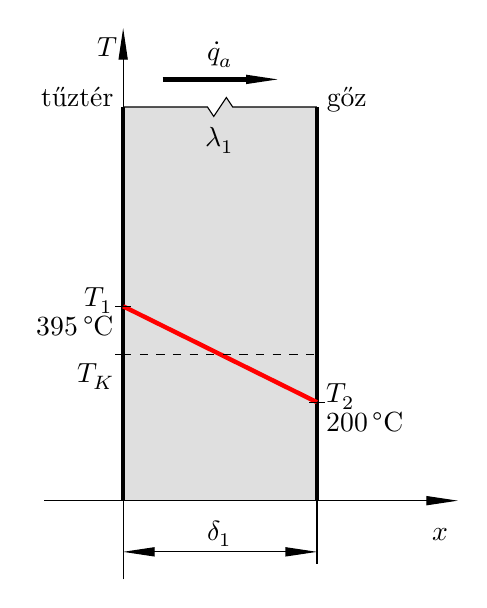
\begin{tikzpicture}
			\pgfmathsetmacro{\d}{16/6.5}
			\pgfmathsetmacro{\L}{5}
			\pgfmathsetmacro{\TA}{395/160}
			\pgfmathsetmacro{\TB}{200/160}
			\pgfmathsetmacro{\TK}{(\TA+\TB)/2}
			
			% Fal
			\fill[gray,opacity=0.25] (0,0) -- (0,\L) -- ({\d/2-0.16},\L) -- ({\d/2-0.08}, {\L-0.12}) -- ({\d/2+0.08}, {\L +0.12}) -- ({\d/2+0.16}, \L) -- (\d, \L) -- (\d, 0);
			\draw[] (0,\L) -- ({\d/2-0.16},\L) -- ({\d/2-0.08}, {\L-0.12}) -- ({\d/2+0.08}, {\L+0.12}) -- ({\d/2+0.16}, \L) -- (\d, \L);
			\draw[ultra thick] (0,0) -- (0,\L);
			\draw[ultra thick] (\d, 0) -- (\d, \L);
			
			% Feliratok
			\node[anchor=base east] at (0, \L) {tűztér};
			\node[anchor=base west] at (\d, \L) {gőz};
			
			% Tengelyek
			\draw[->] (0,-1) -- (0,\L+1) node[anchor=north east]{$T$};
			\draw[->] (-1,0) -- (4.25,0) node[anchor=base east, shift={(0,-0.5)}]{$x$};
			
			% Hőáram és hőáramsűrűség
			\draw[->, ultra thick] (0.5,{\L+0.35}) -- ({\d/2},{\L+0.35}) node[anchor=south]{$\dot{q}_a$} -- ({\d - 0.5},{\L+0.35});
			
			% A hővezetési tényező
			\node[anchor=base] at ({\d/2},{\L-0.5}) {$\lambda_1$};
			
			% T(x)
			\draw[red, ultra thick] (0,\TA) -- (\d,\TB);
			
			% A delta_1 falvastagság
			\pgflength[xa=0, ya=0, xb=\d, yb=0, alim=0]{$\delta_1$};
			
			% A hőmérséklet értékek
			\draw (-0.1,\TA) -- (0.1,\TA);
			\node[anchor=base east] at (0,\TA) {$T_1$};
			\node[anchor=north east] at (0,\TA) {$\SI{395}{\celsius}$};
			
			\draw (-0.1+\d,\TB) -- (0.1+\d,\TB);
			\node[anchor=base west] at (\d,\TB) {$T_2$};
			\node[anchor=north west] at (\d,\TB) {$\SI{200}{\celsius}$};
			
			% A közepes hőmérséklet
			\draw[dashed] (0,\TK) -- (\d,\TK);
			\draw (-0.1,\TK) -- (0.1,\TK);
			\node[anchor=north east] at (0,\TK) {$T_K$};
			
		\end{tikzpicture}
		\caption{A hőmérséklet-hely függvény az a) esetben.}
	\end{subfigure}
	\begin{subfigure}[b]{0.31\textwidth}
		\centering
		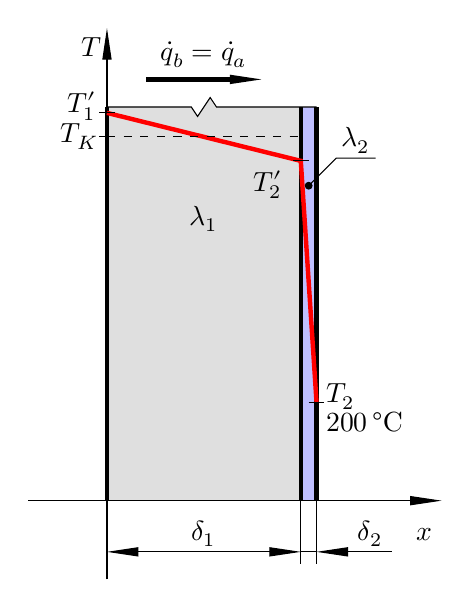
\begin{tikzpicture}
			\pgfmathsetmacro{\d}{16/6.5}
			\pgfmathsetmacro{\v}{1.2/6}
			\pgfmathsetmacro{\L}{5}
			\pgfmathsetmacro{\TA}{788/160}
			\pgfmathsetmacro{\TB}{690.5/160}
			\pgfmathsetmacro{\TC}{200/160}
			\pgfmathsetmacro{\TK}{(\TA+\TB)/2}
			
			% Fal
			\fill[gray,opacity=0.25] (0,0) -- (0,\L) -- ({\d/2-0.16},\L) -- ({\d/2-0.08}, {\L-0.12}) -- ({\d/2+0.08}, {\L +0.12}) -- ({\d/2+0.16}, \L) -- (\d, \L) -- (\d, 0);
			\fill[blue,opacity=0.25] (\d, \L) -- (\d, 0) -- (\d+\v, 0) -- (\d+\v, \L);
			\draw[] (0,\L) -- ({\d/2-0.16},\L) -- ({\d/2-0.08}, {\L-0.12}) -- ({\d/2+0.08}, {\L+0.12}) -- ({\d/2+0.16}, \L) -- (\d, \L) -- (\d+\v, \L);
			\draw[ultra thick] (0,0) -- (0,\L);
			\draw[ultra thick] (\d, 0) -- (\d, \L);
			\draw[ultra thick] (\d+\v, 0) -- (\d+\v, \L);
			
			% Tengelyek
			\draw[->] (0,-1) -- (0,\L+1) node[anchor=north east]{$T$};
			\draw[->] (-1,0) -- (4.25,0) node[anchor=base east, shift={(0,-0.5)}]{$x$};
			
			% Hőáram és hőáramsűrűség
			\draw[->, ultra thick] (0.5,{\L+0.35}) -- ({\d/2},{\L+0.35}) node[anchor=south]{$\dot{q}_b = \dot{q}_a$} -- ({\d - 0.5},{\L+0.35});
			
			% A hővezetési tényező
			\node[anchor=base] at ({\d/2},{\L-1.5}) {$\lambda_1$};
			\node[anchor=base] at ({\d+\v+0.5},{\L-0.5}) {$\lambda_2$};
			\draw ({\d+\v+0.75},{\L-0.65}) -- ({\d+\v+0.25},{\L-0.65}) -- ({\d+\v/2},{\L-1});
			\fill[] ({\d+\v/2},{\L-1}) circle[radius=0.05];
			
			% A falvastagságok
			\pgflength[xa=0, ya=0, xb=\d, yb=0, alim=0]{$\delta_1$};
			\pgflength[xa=\d, ya=0, xb=\d+\v, yb=0, alim=0, a=0, belül=2]{$\delta_2$};
			
			% T(x)
			\draw[red, ultra thick] (0,\TA) -- (\d,\TB) -- (\d+\v,\TC);
			
			% Falhőmérsékletek
			\draw (-0.1,\TA) -- (0.1,\TA);
			\node[anchor=base east] at (0,\TA) {$T_1'$};
			
			\draw (-0.1+\d,\TB) -- (0.1+\d,\TB);
			\node[anchor=north east] at (\d-0.1,\TB) {$T_2'$};
			
			\draw (-0.1+\d+\v,\TC) -- (0.1+\d+\v,\TC);
			\node[anchor=base west] at (\d+\v,\TC) {$T_2$};
			\node[anchor=north west] at (\d+\v,\TC) {$\SI{200}{\celsius}$};
			
			% A közepes hőmérséklet
			\draw[dashed] (0,\TK) -- (\d,\TK);
			\draw (-0.1,\TK) -- (0.1,\TK);
			\node[anchor=east] at (0,\TK) {$T_K$};
			
		\end{tikzpicture}
		\caption{A hőmérséklet-hely függvény az b) esetben.}
	\end{subfigure}
	\begin{subfigure}[b]{0.31\textwidth}
		\centering
		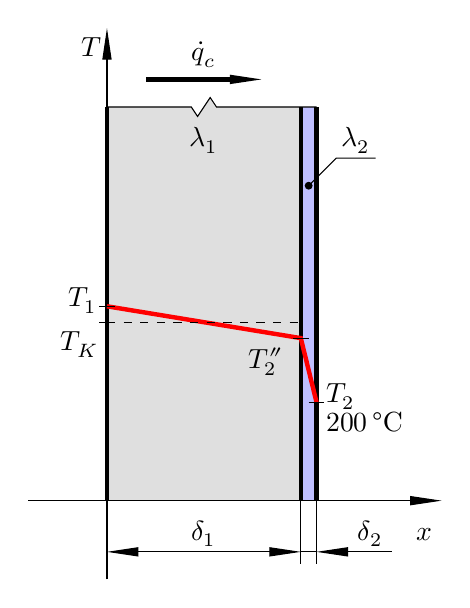
\begin{tikzpicture}
			\pgfmathsetmacro{\d}{16/6.5}
			\pgfmathsetmacro{\v}{1.2/6}
			\pgfmathsetmacro{\L}{5}
			\pgfmathsetmacro{\TA}{395/160}
			\pgfmathsetmacro{\TB}{330.3/160}
			\pgfmathsetmacro{\TC}{200/160}
			\pgfmathsetmacro{\TK}{(\TA+\TB)/2}
			
			% Fal
			\fill[gray,opacity=0.25] (0,0) -- (0,\L) -- ({\d/2-0.16},\L) -- ({\d/2-0.08}, {\L-0.12}) -- ({\d/2+0.08}, {\L +0.12}) -- ({\d/2+0.16}, \L) -- (\d, \L) -- (\d, 0);
			\fill[blue,opacity=0.25] (\d, \L) -- (\d, 0) -- (\d+\v, 0) -- (\d+\v, \L);
			\draw[] (0,\L) -- ({\d/2-0.16},\L) -- ({\d/2-0.08}, {\L-0.12}) -- ({\d/2+0.08}, {\L+0.12}) -- ({\d/2+0.16}, \L) -- (\d, \L) -- (\d+\v, \L);
			\draw[ultra thick] (0,0) -- (0,\L);
			\draw[ultra thick] (\d, 0) -- (\d, \L);
			\draw[ultra thick] (\d+\v, 0) -- (\d+\v, \L);
			
			% Tengelyek
			\draw[->] (0,-1) -- (0,\L+1) node[anchor=north east]{$T$};
			\draw[->] (-1,0) -- (4.25,0) node[anchor=base east, shift={(0,-0.5)}]{$x$};
			
			% Hőáram és hőáramsűrűség
			\draw[->, ultra thick] (0.5,{\L+0.35}) -- ({\d/2},{\L+0.35}) node[anchor=south]{$\dot{q}_c$} -- ({\d - 0.5},{\L+0.35});
			
			% A hővezetési tényező
			\node[anchor=base] at ({\d/2},{\L-0.5}) {$\lambda_1$};
			\node[anchor=base] at ({\d+\v+0.5},{\L-0.5}) {$\lambda_2$};
			\draw ({\d+\v+0.75},{\L-0.65}) -- ({\d+\v+0.25},{\L-0.65}) -- ({\d+\v/2},{\L-1});
			\fill[] ({\d+\v/2},{\L-1}) circle[radius=0.05];
			
			% A falvastagságok
			\pgflength[xa=0, ya=0, xb=\d, yb=0, alim=0]{$\delta_1$};
			\pgflength[xa=\d, ya=0, xb=\d+\v, yb=0, alim=0, a=0, belül=2]{$\delta_2$};
			
			% T(x)
			\draw[red, ultra thick] (0,\TA) -- (\d,\TB) -- (\d+\v,\TC);
			
			% Falhőmérsékletek
			\draw (-0.1,\TA) -- (0.1,\TA);
			\node[anchor=base east] at (0,\TA) {$T_1$};
			%\node[anchor=north east] at (0,\TA) {$\SI{395}{\celsius}$};
			
			\draw (-0.1+\d,\TB) -- (0.1+\d,\TB);
			\node[anchor=north east] at (\d-0.1,\TB) {$T_2''$};
			
			\draw (-0.1+\d+\v,\TC) -- (0.1+\d+\v,\TC);
			\node[anchor=base west] at (\d+\v,\TC) {$T_2$};
			\node[anchor=north west] at (\d+\v,\TC) {$\SI{200}{\celsius}$};
			
			% A közepes hőmérséklet
			\draw[dashed] (0,\TK) -- (\d,\TK);
			\draw (-0.1,\TK) -- (0.1,\TK);
			\node[anchor=north east] at (0,\TK) {$T_K$};
			
		\end{tikzpicture}
		\caption{A hőmérséklet-hely függvény a c) esetben.}
	\end{subfigure}
\end{figure}

\subsubsection*{a) Határozzuk meg a fal közepes hőmérsékletét és a falban kialakuló hőáramsűrűséget!}

A fal közepes hőmérséklete a lineáris hőmérsékleteloszlás miatt a falhőmérsékletek átlaga:
\begin{equation}
	T_K = \frac{T_1 + T_2}{2} = \SI{297.5}{\celsius}
\end{equation}

Nem lineáris hőmérsékleteloszlás esetén a hőmérséklet-hely függvény határozott integráljának és a falvastagságnak a hányadosa a közepes hőmérséklet.

A hőáramsűrűség a falban
\begin{equation}
	\dot{q}_a = \frac{\lambda_1}{\delta_1} (T_1 - T_2) = \SI{524}{\kilo\watt\per\meter\squared}
\end{equation}
Ebben a feladatban a kazánfal oldalain végbemenő hőátadást tökéletesnek tekintjük, azaz a falhőmérsékletek megegyeznek a közeghőmérsékletekkel.

\subsubsection*{b) A kazán falára $\delta_2 = \SI{1.2}{\milli\meter}$ vastag kazánkőréteg rakódik. Változatlan gőztermelés és gőznyomás esetén számítsuk ki a kazán falának közepes hőmérsékletét!}

A vízkőréteg hővezetési tényezője $\lambda_2 = \SI{1.6}{\watt\per\meter\kelvin}$.

\vspace{2mm}

A "változatlan gőztermelés" kifejezés azt jelenti, hogy a gőzoldali falhőmérséklet és a hőáramsűrűség a falban nem változik. A vízkőréteg miatt a hőáramsűrűség csak úgy maradhat azonos $\dot{q}_a$-val, hogy a tűztér oldali $T_1'$ falhőmérséklet sokkal nagyobb $T_1$-nél, a $T_2'$ falhőmérséklet pedig nem azonos a gőzoldali $T_2$ hőmérséklettel. A vízkőréteg hővezetési tényezője sokkal kisebb a kazánlemezénél, ezért a kisebb rétegvastagság ellenére nagyobb hőmérséklet esik rajta.

A fal közepes hőmérséklete itt is a két falhőmérséklet átlaga:
\begin{equation}
	T_K' = \frac{T_1' + T_2'}{2}
\end{equation}

A $T_1'$ és a $T_2'$ falhőmérséklet a $q_b$ hőáramsűrűség alapján számítható ki:
\begin{equation}
	\dot{q}_b = \dot{q}_a = \frac{\lambda_1}{\delta_1} (T_1' - T_2') = \frac{\lambda_2}{\delta_2} (T_2' - T_2)
\end{equation}

\begin{equation}
	T_2' = T_2 + \frac{\delta_2}{\lambda_2}\dot{q}_a = \SI{200}{\celsius} + \frac{\SI{1.2}{\milli\meter}}{\SI{1.6}{\watt\per\meter\kelvin}} \SI{524}{\kilo\watt\per\meter\squared} = \SI{593}{\celsius}
\end{equation}

\begin{equation}
	T_1' = T_2' + \frac{\delta_1}{\lambda_1}\dot{q}_a = \SI{593}{\celsius} + \frac{\SI{16}{\milli\meter}}{\SI{43}{\watt\per\meter\kelvin}} \SI{524}{\kilo\watt\per\meter\squared} = \SI{788}{\celsius}
\end{equation}

\subsubsection*{c) Ha szilárdsági okok miatt a fal hőmérséklete nem emelkedhet, de a gőznyomás változatlan, mekkora lesz a hőáramsűrűség?}

Ha gőznyomás nem változik, akkor a gőz hőmérséklete sem változik, mivel a kazánban a nedves gőzmezőbe eső állapotú a víz, és ott T--s diagram szerint az izotermák és az izobár vonalak egybeesnek. Tehát a gőzoldali hőmérséklet $T_2$. Ha szilárdsági okok miatt a fal hőmérséklete nem emelkedhet, akkor a tűztér oldali hőmérséklet az eredeti $T_1$.

A $\dot{q}_c$ hőáramsűrűség azonos a kazánfalban és a vízkőrétegben:
\begin{equation}
	\dot{q}_c = \frac{\lambda_1}{\delta_1} (T_1 - T_2'') = \frac{\lambda_2}{\delta_2} (T_2'' - T_2)
\end{equation}

Kifejezve a két hőmérsékletkülönbséget, és összeadva a két egyenletet:
\begin{equation}
	\left.
	\begin{array}{lcl}
		\dot{q}_c \dfrac{\delta_1}{\lambda_1} = (T_1 - T_2'') \\
		\dot{q}_c \dfrac{\delta_2}{\lambda_2} = (T_2'' - T_2)
	\end{array}
	\right\rbrace
	\quad \Rightarrow \quad 
	\dot{q}_c \left(\dfrac{\delta_1}{\lambda_1} + \dfrac{\delta_2}{\lambda_2} \right) = (T_1 - T_2) 
	\quad \Rightarrow \quad 
	\dot{q}_c = 
	\SI{173.78}{\kilo\watt\per\meter\squared}
\end{equation}

A fenti két egyenletet kétismeretlenes egyenletrendszernek is tekinthetjük, ahol a hőáramsűrűség mellett a másik ismeretlen a $T_2''$ falhőmérséklet. A hőáramsűrűséget visszahelyettesítve megkaphatjuk az értékét:
\begin{equation}
	T_2'' = T_1 - \dot{q}_c \dfrac{\delta_1}{\lambda_1} = \SI{330.34}{\celsius}
\end{equation}

\pagebreak



% K5/2-es feladat


\section*{K5/2. feladat}
\addcontentsline{toc}{section}{K5/2. feladat}
Egy NÁ125-ös szénacél csőben (a külső átmérő $d_2 = \SI{133}{\milli\meter}$, a belső átmérő $d_1 = \SI{125}{\milli\meter}$, a falvastagság $s = \SI{4}{\milli\meter}$) ammóniát szállítanak, amelynek nyomása $p = \SI{2.9}{\bar}$, hőmérséklete $T_1 = \SI{-10}{\celsius}$.

A környezet levegője ($T_4 = \SI{+10}{\celsius}$) melegíti a csövet, ammónia forrásban van a cső belsejében, így belülről hőelvonás van, és a cső hideg külső felületére kifagy a levegő nedvességtartalma. A kifagyott jégréteg szigetelőként működik, beáll az egyensúlyi állapot.

Meghatározandó a csőre fagyott jégréteg külső $d_3$ átmérője! A jégréteg felületének hőmérséklete $T_3 = \SI{0}{\celsius}$ (olvadó jég), a csőfal belső hőmérséklete pedig a forrásban lévő ammónia jó hőátadási tényezője miatt $T_1 = \SI{-10}{\celsius}$-nak vehető (a hőátadás termikus ellenállása elhanyagolható).

\begin{figure}[h]
	\centering
	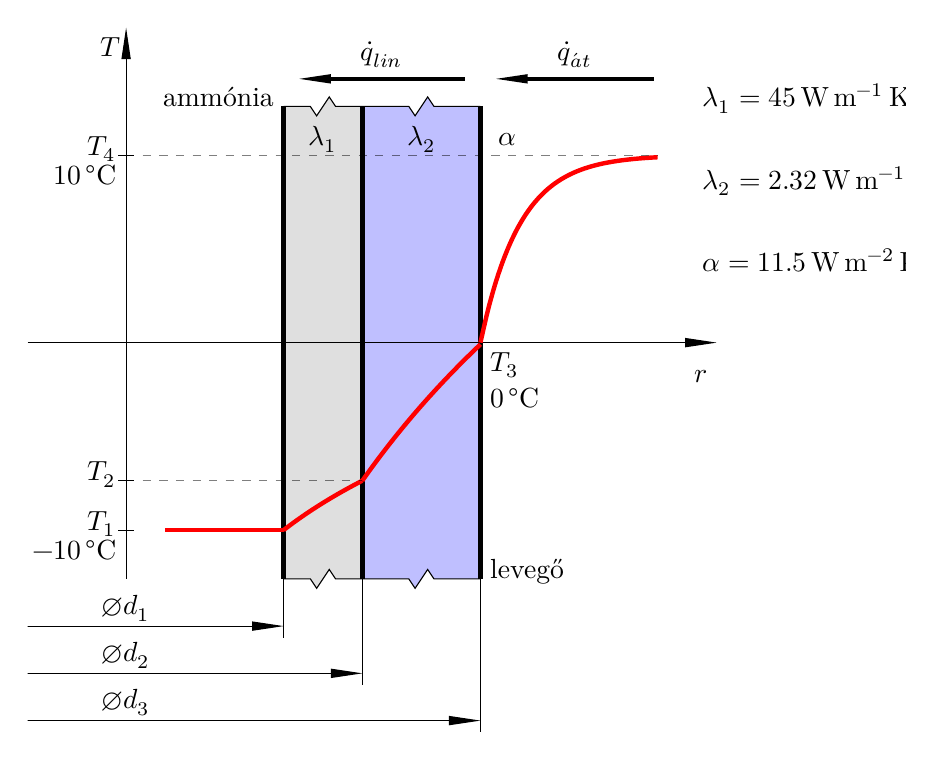
\begin{tikzpicture}
		% Fiktív értékek a vázlathoz
		\pgfmathsetmacro{\DB}{4}
		\pgfmathsetmacro{\DK}{6}
		\pgfmathsetmacro{\DJ}{9}
		\pgfmathsetmacro{\lambdaA}{8}
		\pgfmathsetmacro{\lambdaJ}{2.9}
		\pgfmathsetmacro{\alfaL}{11.5}
		\pgfmathsetmacro{\qlin}{326.815}
		
		\pgfmathsetmacro{\RA}{\DB/2}
		\pgfmathsetmacro{\RB}{\DK/2}
		\pgfmathsetmacro{\RC}{\DJ/2}
		
		\pgfmathsetmacro{\L}{3}
		
		\pgfmathsetmacro{\kelvin}{4.2}
		\pgfmathsetmacro{\TA}{-10/\kelvin}
		\pgfmathsetmacro{\TB}{-7.36/\kelvin}
		\pgfmathsetmacro{\TC}{0/\kelvin}
		\pgfmathsetmacro{\TD}{10/\kelvin}
		
		% KÖRBEVÁGÁS
		\clip ({-1.25}, {-(\L)-2}) rectangle ({2.2*\RC}, {\L+1});
		
		% A csőfal és a jégréteg
		\fill[gray, opacity=0.25] (\RA,\L) -- ({(\RA+\RB)/2-0.16},\L) -- ({(\RA+\RB)/2-0.08}, {\L-0.12}) -- ({(\RA+\RB)/2+0.08}, {\L+0.12}) -- ({(\RA+\RB)/2+0.16}, \L) -- (\RB, \L) -- (\RB, -\L) -- ({(\RA+\RB)/2+0.16}, -\L) -- ({(\RA+\RB)/2+0.08}, {-\L+0.12}) -- ({(\RA+\RB)/2-0.08}, {-\L-0.12}) -- ({(\RA+\RB)/2-0.16},-\L) -- (\RA,-\L);
		\draw[] (\RA,\L) -- ({(\RA+\RB)/2-0.16},\L) -- ({(\RA+\RB)/2-0.08}, {\L-0.12}) -- ({(\RA+\RB)/2+0.08}, {\L+0.12}) -- ({(\RA+\RB)/2+0.16}, \L) -- (\RB, \L);
		\draw[] (\RA,-\L) -- ({(\RA+\RB)/2-0.16},-\L) -- ({(\RA+\RB)/2-0.08}, {-\L-0.12}) -- ({(\RA+\RB)/2+0.08}, {-\L+0.12}) -- ({(\RA+\RB)/2+0.16}, -\L) -- (\RB, -\L);
		
		\fill[blue, opacity=0.25] (\RB,\L) -- ({(\RB+\RC)/2-0.16},\L) -- ({(\RB+\RC)/2-0.08}, {\L-0.12}) -- ({(\RB+\RC)/2+0.08}, {\L+0.12}) -- ({(\RB+\RC)/2+0.16}, \L) -- (\RC, \L) -- (\RC, -\L) -- ({(\RB+\RC)/2+0.16}, -\L) -- ({(\RB+\RC)/2+0.08}, {-\L+0.12}) -- ({(\RB+\RC)/2-0.08}, {-\L-0.12}) -- ({(\RB+\RC)/2-0.16},-\L) -- (\RB,-\L);
		\draw[] (\RB,\L) -- ({(\RB+\RC)/2-0.16},\L) -- ({(\RB+\RC)/2-0.08}, {\L-0.12}) -- ({(\RB+\RC)/2+0.08}, {\L+0.12}) -- ({(\RB+\RC)/2+0.16}, \L) -- (\RC, \L);
		\draw[] (\RB,-\L) -- ({(\RB+\RC)/2-0.16},-\L) -- ({(\RB+\RC)/2-0.08}, {-\L-0.12}) -- ({(\RB+\RC)/2+0.08}, {-\L+0.12}) -- ({(\RB+\RC)/2+0.16}, -\L) -- (\RC, -\L);
		
		\draw[ultra thick] (\RA,-\L) -- (\RA,\L);
		\draw[ultra thick] (\RB,-\L) -- (\RB,\L);
		\draw[ultra thick] (\RC,-\L) -- (\RC,\L);
		
		% Tengelyek
		\draw[->] (0,-\L) -- (0,\L+1) node[anchor=north east]{$T$};
		\draw[->] (-1.25, 0) -- (\RC+3, 0) node[anchor=base east, shift={(0,-0.5)}]{$r$};
		
		% Hőáram és hőáramsűrűség
		\draw[->, ultra thick] (\RC-0.2,{\L+0.35}) -- ({(\RA+\RC)/2},{\L+0.35}) node[anchor=south]{$\dot{q}_{lin}$} -- (\RA+0.2,{\L+0.35});
		\draw[->, ultra thick] (\RC+2.2,{\L+0.35}) -- (\RC+1.2,{\L+0.35}) node[anchor=south]{$\dot{q}_{\acute{a}t}$} -- (\RC+0.2,{\L+0.35});
		
		% A hővezetési és hőátadási tényezők
		\node[anchor=base] at ({(\RA+\RB)/2},{\L-0.5}) {$\lambda_1$};
		\node[anchor=base] at ({(\RB+\RC)/2},{\L-0.5}) {$\lambda_2$};
		\node[anchor=base west] at ({(\RC+0.1},{\L-0.5}) {$\alpha$};
		
		% Az átmérők
		\pgflength[xa={-\RA}, ya={-\L}, xb={\RA}, yb={-\L}, alim=0, blim=1, ra=0.6]{$\diameter d_1$};
		\pgflength[xa={-\RB}, ya={-\L}, xb={\RB}, yb={-\L}, alim=0, blim=1, ra=1.2]{$\diameter d_2$};
		\pgflength[xa={-\RC}, ya={-\L}, xb={\RC}, yb={-\L}, alim=0, blim=1, ra=1.8]{$\diameter d_3$};
		
		% T(r) körülbelüli hőmérséklet-hely függvény
		\draw[red, ultra thick] (0.5,\TA) -- (\RA,\TA);
		\draw[ultra thick, color=red, domain=\RA:\RB, smooth, variable=\r] plot (\r, {\TA + ( \qlin/(2*3.14159*\lambdaA) * ln(2*\r/\DB))/\kelvin});
		\draw[ultra thick, color=red, domain=\RB:\RC, smooth, variable=\r] plot (\r, {\TA + (\qlin/(2*3.14159*\lambdaA) * ln(\DK/\DB) + \qlin/(2*3.14159*\lambdaJ) * ln(2*\r/\DK))/\kelvin});
		
		\draw[ultra thick, color=red, domain=\RC:1.5*\RC, smooth, variable=\r] plot (\r, {\TD * (1-exp(-(\r-\RC)/0.5))});
		
		% A hőmérséklet értékek
		\draw (-0.1,\TA) -- (0.1,\TA);
		\node[anchor=base east] at (0,\TA) {$T_1$};
		\node[anchor=north east] at (0,\TA) {$\SI{-10}{\celsius}$};
		
		\draw (-0.1,\TB) -- (0.1,\TB);
		\draw[black, opacity=0.5, dashed] (0,\TB) -- (\RB,\TB);
		\node[anchor=base east] at (0,\TB) {$T_2$};
		
		\draw (-0.1,\TD) -- (0.1,\TD);
		\draw[black, opacity=0.5, dashed] (0,\TD) -- (1.5*\RC,\TD);
		\node[anchor=base east] at (0,\TD) {$T_4$};
		\node[anchor=north east] at (0,\TD) {$\SI{10}{\celsius}$};
		
		\node[anchor=north west] at (\RC,\TC) {$T_3$};
		\node[anchor=north west] at (\RC, -0.45) {$\SI{0}{\celsius}$};
		
		% Feliratok
		\node[anchor=base east] at (\RA, \L) {ammónia};
		\node[anchor=base west] at (\RC, -\L) {levegő};
		
		% Adatok
		\node[anchor=base west] at (1.6*\RC, \L) {$\lambda_1 = \SI{45}{\watt\per\meter\kelvin}$};
		\node[anchor=base west] at (1.6*\RC, 0.65*\L) {$\lambda_2 = \SI{2.32}{\watt\per\meter\kelvin}$};
		\node[anchor=base west] at (1.6*\RC, 0.3*\L) {$\alpha = \SI{11.5}{\watt\per\meter\squared\kelvin}$};
		
	\end{tikzpicture}
	\caption{A hőmérséklet-hely függvény \textbf{nem méretarányos} vázlata.}
\end{figure}

\subsubsection*{Vizsgálat többrétegű hengeres falként}
A csőfal és a rárakódó jégréteg hengeres alakú, ezért lineáris a hőáramsűrűségeket tudjuk felírni. A csőfalban és a jégrétegben állandósult a hőmérsékleteloszlás és csak hővezetés történik. A hengeres falakra a $\dot{q}_{lin}$ \textbf{vezetéses} lineáris hőáramsűrűség vonatkozik.
\begin{equation}
	\dot{q}_{lin} = \dfrac{T_3 - T_1}{\dfrac{\ln\frac{d_2}{d_1}}{2 \pi \lambda_1} + \dfrac{\ln\frac{d_3}{d_2}}{2 \pi \lambda_2}}
\end{equation}

A levegőből a jégrétegbe \textbf{átadódó} $\dot{q}_{\acute{a}t}$ lineáris hőáramsűrűség: 
\begin{equation}
	\dot{q}_{\acute{a}t} = \alpha d_3 \pi (T_4 - T_3)
\end{equation}

A két lineáris hőáramsűrűséget az ábrán úgy vettük fel, hogy a hőmérsékletcsökkenés irányába pozitívak, ezért a felírásuknál a nagyobb hőmérsékletből vonjuk ki a kisebbet.

Az energiamegmaradás miatt a két lineáris hőáramsűrűség egyenlő:
\begin{equation}
	\dot{q}_{lin} = \dot{q}_{\acute{a}t} = \dot{q}
\end{equation}

A fentiekből az alábbi kétismeretlenes egyenletrendszert kapjuk, amiben a jégréteg $d_3$ átmérője a a $\dot{q}$ lineáris hőáramsűrűség az ismeretlenek. Az egyenletrendszer nem lineáris, átrendezéssel nem oldható meg (transzcendens), csak numerikus közelítő megoldása lehetséges:
\begin{equation}
	\left.
	\begin{array}{lcl}
		\dot{q} = \dfrac{T_3 - T_1}{\dfrac{\ln\frac{d_2}{d_1}}{2 \pi \lambda_1} + \dfrac{\ln\frac{d_3}{d_2}}{2 \pi \lambda_2}} \\ \\
		\dot{q} = \alpha d_3 \pi (T_4 - T_3)
	\end{array}
	\right\rbrace
	\quad \Rightarrow \quad 
	\left\lbrace
	\begin{array}{lcl}
		\dot{q} \approx \SI{137.873}{\watt\per\meter} \\ \\
		d_3 \approx \SI{381.6}{\milli\meter}
	\end{array}
	\right.
\end{equation}

Innen a jégréteg vastagsága $\dfrac{1}{2}\left(d_3 - d_2\right) = \SI{124.3}{\milli\meter}$.

\subsubsection*{A méretarányos ábra és a hőmérséklet hely függvény}
A lineáris hőáramsűrűség és a jég külső átmérőjének numerikus közelítő megoldását felhasználva megrajzolható méretarányosan a $T\!\left(r\right)$ hőmérséklet-hely függvény. A hőmérséklet a $d_1$ átmérőn belül állandó $T_1$ érték. A csőfalban és a jégrétegben $T\!\left(r\right) = T_0 + \dfrac{\dot{q}}{2 \pi \lambda} \ln\dfrac{r}{r_0}$ alakban írható fel, ahol a $T_0$ a belső $r_0$ sugárhoz tartozó hőmérséklet.

A csőfal esetén $T_0 = T_1$ és $r_0 = \dfrac{d_1}{2}$:
\begin{equation}
	T\!\left(r\right) = T_1 + \dfrac{\dot{q}}{2 \pi \lambda_1} \ln\dfrac{2 r}{d_1}
\end{equation}

Innen megkaphatjuk a csőfal és a jégréteg határfelületének hőmértékletét, $T_2$-t:
\begin{equation}
	T_2 = T\!\left(\frac{d_2}{2}\right) = T_1 + \dfrac{\dot{q}}{2 \pi \lambda_1} \ln\dfrac{d_2}{d_1} = \SI{-9.96}{\celsius}
\end{equation}

A jégréteg esetén $T_0 = T_2$ és $r_0 = \dfrac{d_2}{2}$:
\begin{equation}
	T\!\left(r\right) = T_2 + \dfrac{\dot{q}}{2 \pi \lambda_2} \ln\dfrac{2 r}{d_2}
\end{equation}

\begin{figure}[h]
	\centering
	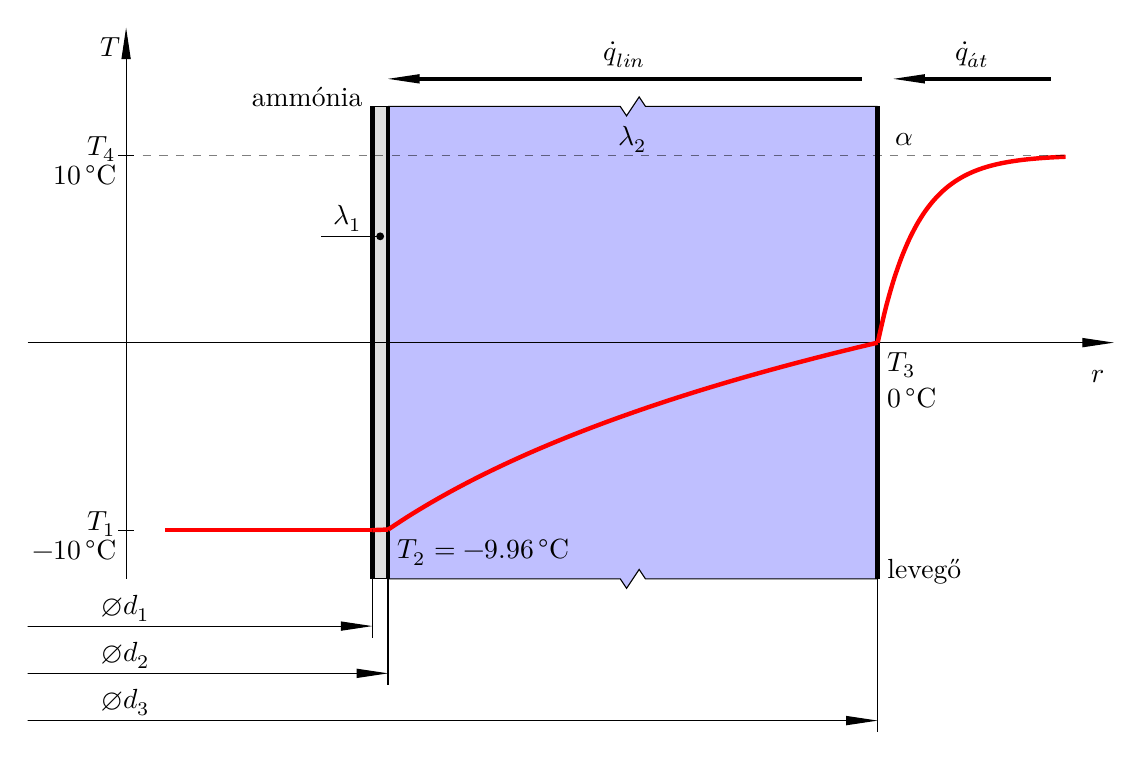
\begin{tikzpicture}
	% Fiktív értékek a vázlathoz
	\pgfmathsetmacro{\meter}{1/50}
	\pgfmathsetmacro{\DB}{0.125/\meter}
	\pgfmathsetmacro{\DK}{0.133/\meter}
	\pgfmathsetmacro{\DJ}{0.3816/\meter}
	\pgfmathsetmacro{\lambdaA}{45}
	\pgfmathsetmacro{\lambdaJ}{2.32}
	\pgfmathsetmacro{\alfaL}{11.5}
	\pgfmathsetmacro{\qlin}{137.873}
	
	\pgfmathsetmacro{\RA}{\DB/2}
	\pgfmathsetmacro{\RB}{\DK/2}
	\pgfmathsetmacro{\RC}{\DJ/2}
	
	\pgfmathsetmacro{\L}{3}
	
	\pgfmathsetmacro{\kelvin}{4.2}
	\pgfmathsetmacro{\TA}{-10/\kelvin}
	\pgfmathsetmacro{\TB}{-9.96/\kelvin}
	\pgfmathsetmacro{\TC}{0/\kelvin}
	\pgfmathsetmacro{\TD}{10/\kelvin}
	
	% KÖRBEVÁGÁS
	\clip ({-1.25}, {-(\L)-2}) rectangle ({1.32*\RC}, {\L+1});
	
	% A csőfal és a jégréteg
	\fill[gray,opacity=0.25] (\RA,\L) -- (\RB, \L) -- (\RB, -\L) -- (\RA,-\L);
	\draw[] (\RA,\L) -- (\RB, \L);
	\draw[] (\RA,-\L) -- (\RB, -\L);
	
	\fill[blue,opacity=0.25] (\RB,\L) -- ({(\RB+\RC)/2-0.16},\L) -- ({(\RB+\RC)/2-0.08}, {\L-0.12}) -- ({(\RB+\RC)/2+0.08}, {\L+0.12}) -- ({(\RB+\RC)/2+0.16}, \L) -- (\RC, \L) -- (\RC, -\L) -- ({(\RB+\RC)/2+0.16}, -\L) -- ({(\RB+\RC)/2+0.08}, {-\L+0.12}) -- ({(\RB+\RC)/2-0.08}, {-\L-0.12}) -- ({(\RB+\RC)/2-0.16},-\L) -- (\RB,-\L);
	\draw[] (\RB,\L) -- ({(\RB+\RC)/2-0.16},\L) -- ({(\RB+\RC)/2-0.08}, {\L-0.12}) -- ({(\RB+\RC)/2+0.08}, {\L+0.12}) -- ({(\RB+\RC)/2+0.16}, \L) -- (\RC, \L);
	\draw[] (\RB,-\L) -- ({(\RB+\RC)/2-0.16},-\L) -- ({(\RB+\RC)/2-0.08}, {-\L-0.12}) -- ({(\RB+\RC)/2+0.08}, {-\L+0.12}) -- ({(\RB+\RC)/2+0.16}, -\L) -- (\RC, -\L);
	
	\draw[ultra thick] (\RA,-\L) -- (\RA,\L);
	\draw[ultra thick] (\RB,-\L) -- (\RB,\L);
	\draw[ultra thick] (\RC,-\L) -- (\RC,\L);
	
	% Tengelyek
	\draw[->] (0,-\L) -- (0,\L+1) node[anchor=north east]{$T$};
	\draw[->] (-1.25, 0) -- (\RC+3, 0) node[anchor=base east, shift={(0,-0.5)}]{$r$};
	
	% Hőáram és hőáramsűrűség
	\draw[->, ultra thick] (\RC-0.2,{\L+0.35}) -- ({(\RA+\RC)/2},{\L+0.35}) node[anchor=south]{$\dot{q}_{lin}$} -- (\RA+0.2,{\L+0.35});
	\draw[->, ultra thick] (\RC+2.2,{\L+0.35}) -- (\RC+1.2,{\L+0.35}) node[anchor=south]{$\dot{q}_{\acute{a}t}$} -- (\RC+0.2,{\L+0.35});
	
	% A hővezetési és hőátadási tényezők
	\node[anchor=base east] at ({\RA},{\L-1.5}) {$\lambda_1$};
	\draw ({\RA-0.65},{\L-1.65}) -- ({(\RA+\RB)/2},{\L-1.65});
	\fill[] ({(\RA+\RB)/2},{\L-1.65}) circle[radius=0.05];
	
	\node[anchor=base] at ({(\RB+\RC)/2},{\L-0.5}) {$\lambda_2$};
	\node[anchor=base west] at ({(\RC+0.1},{\L-0.5}) {$\alpha$};
	
	% Az átmérők
	\pgflength[xa={-\RA}, ya={-\L}, xb={\RA}, yb={-\L}, alim=0, blim=1, ra=0.6]{$\diameter d_1$};
	\pgflength[xa={-\RB}, ya={-\L}, xb={\RB}, yb={-\L}, alim=0, blim=1, ra=1.2]{$\diameter d_2$};
	\pgflength[xa={-\RC}, ya={-\L}, xb={\RC}, yb={-\L}, alim=0, blim=1, ra=1.8]{$\diameter d_3$};
	
	% A T(r) VALÓS hőmérséklet-hely függvény
	\draw[red, ultra thick] (0.5,\TA) -- (\RA,\TA);
	
	\draw[ultra thick, color=red, domain=\RA:\RB, smooth, variable=\r] plot (\r, {\TA + ( \qlin/(2*3.14159*\lambdaA) * ln(2*\r/\DB))/\kelvin});
	
	\draw[ultra thick, color=red, domain=\RB:\RC, smooth, variable=\r] plot (\r, {\TA + (\qlin/(2*3.14159*\lambdaA) * ln(\DK/\DB) + \qlin/(2*3.14159*\lambdaJ) * ln(2*\r/\DK))/\kelvin});
	
	\draw[ultra thick, color=red, domain=\RC:1.25*\RC, smooth, variable=\r] plot (\r, {\TD * (1-exp(-(\r-\RC)/0.5))});
	
	% A hőmérséklet értékek
	\draw (-0.1,\TA) -- (0.1,\TA);
	\node[anchor=base east] at (0,\TA) {$T_1$};
	\node[anchor=north east] at (0,\TA) {$\SI{-10}{\celsius}$};
	
	\node[anchor=north west] at (\RB,\TB) {$T_2 = \SI{-9.96}{\celsius}$};
	
	\draw (-0.1,\TD) -- (0.1,\TD);
	\draw[black, opacity=0.5, dashed] (0,\TD) -- (1.25*\RC,\TD);
	\node[anchor=base east] at (0,\TD) {$T_4$};
	\node[anchor=north east] at (0,\TD) {$\SI{10}{\celsius}$};
	
	\node[anchor=north west] at (\RC,\TC) {$T_3$};
	\node[anchor=north west] at (\RC, -0.45) {$\SI{0}{\celsius}$};
	
	% Feliratok
	\node[anchor=base east] at (\RA, \L) {ammónia};
	\node[anchor=base west] at (\RC, -\L) {levegő};
	
	\end{tikzpicture}
	\caption{A hőmérséklet-hely függvény méretarányosan ábrázolva.}
\end{figure}


A falbeli lineáris hőáram és a hőátadást jellemző lineáris hőáram most is egyenlő. 
\begin{equation}
	\dot{q}_{lin} = \dfrac{T_3 - T_1}{
		\dfrac{d_2-d_1}{\lambda_1\left(d_1+d_2\right) \bcancel{\pi}} + 
		\dfrac{d_3-d_2}{\lambda_2\left(d_2+d_3\right)\bcancel{\pi}}
		}
	= 
	\alpha d_3 \bcancel{\pi} (T_4 - T_3) = \dot{q}_{\acute{a}t}
\end{equation}

Egyszerűsítve, és kifejezve a hőmérsékletkülönbségek hányadosát:
\begin{equation}
	\underbrace{\dfrac{T_3 - T_1}{T_4 - T_3}}_{\substack{T \\ \text{állandó}}}
	= 
	\underbrace{\dfrac{\left(d_2-d_1\right)\alpha}{\lambda_1\left(d_1+d_2\right)}}_{\substack{C \\ \text{állandó}}} d_3
	+ 
	\dfrac{\left(d_3-d_2\right) \alpha d_3}{\lambda_2\left(d_2+d_3\right)}
\end{equation}

Vezessük be a $T$ és $C$ állandókat, hogy gyorsabb és átláthatóbb legyen az egyenlet átrendezése:
\begin{equation}
	T = C d_3 +  \dfrac{\left(d_3-d_2\right) \alpha d_3}{\lambda_2\left(d_2+d_3\right)}
\end{equation}

Megszüntetve a törtet $d_3$-ra másodfokú egyenletet kapunk:
\begin{equation}
	T \lambda_2\left(d_2+d_3\right) = C d_3 \lambda_2\left(d_2+d_3\right) + \left(d_3-d_2\right) \alpha d_3
\end{equation}

\begin{equation}
	\SI{0}{\watt} = \left(C \lambda_2 +\alpha\right)d_3^2 + \left(C \lambda_2 d_2 - d_2 \alpha - T \lambda_2 \right) d_3 - T \lambda_2 d_2
\end{equation}

Innen a $d_3$ közelítő értéke:
\begin{equation}
	d_{3,1} = \SI{0.4008}{\meter}, 
	\quad 
	\underbrace{
		\left(d_{3,2} = \SI{-0.0668}{\meter}\right)
	}_{\substack{\text{a másodfokú egyenletnek megoldása,} \\ \text{de a fizikai problémának nem}}}
\end{equation}

A $d_3$ közelítő megoldással nyert értéke tehát \SI{400.8}{\milli\meter}. A nemlineáris egyenlet közelítő numerikus megoldásától ez 5\,\%-kal tér el.

\pagebreak


% K5/3-as feladat


% K5/4-es feladat


\section*{K5/4. feladat: Hengeres fal közelítése síkfallal}
\addcontentsline{toc}{section}{K5/4. feladat: Hengeres fal közelítése síkfallal}

\begin{tabular}{ | p{2cm} | p{14cm} | } 
	\hline
	Név & Szalay István \\ 
	\hline
	Szak & \\ 
	\hline
	Félév & 2019/2020 II. (tavaszi) félév \\ 
	\hline
\end{tabular}
\vspace{0.5cm}

\noindent Gyakorlati számítások során szokás a hengeres falon vezetéssel átjutó hőáramot közelítő módon síkfalra vonatkozó összefüggésekkel számolni. Határozza meg egy hengeres fal külső $d_2$ és belső $d_1$ átmérőjének hányadosa függvényében, hogy a lineáris hőáramsűrűség számításakor hány \%-os hibát vétünk az alábbi közelítő összefüggéseket használva:
\begin{equation}
	\dot{q}_{lin} = \dfrac{\lambda}{\delta} d_K \pi \left(T_1 - T_2\right),
	\quad 
	\delta = \dfrac{d_2 - d_1}{2}, 
	\quad 
	\text{és} 
	\quad d_K = \dfrac{d_1 + d_2}{2}
\end{equation}

ahol $\delta$ a falvastagság és $d_K$ a közepes átmérő.


\begin{figure}[h]
	\centering
	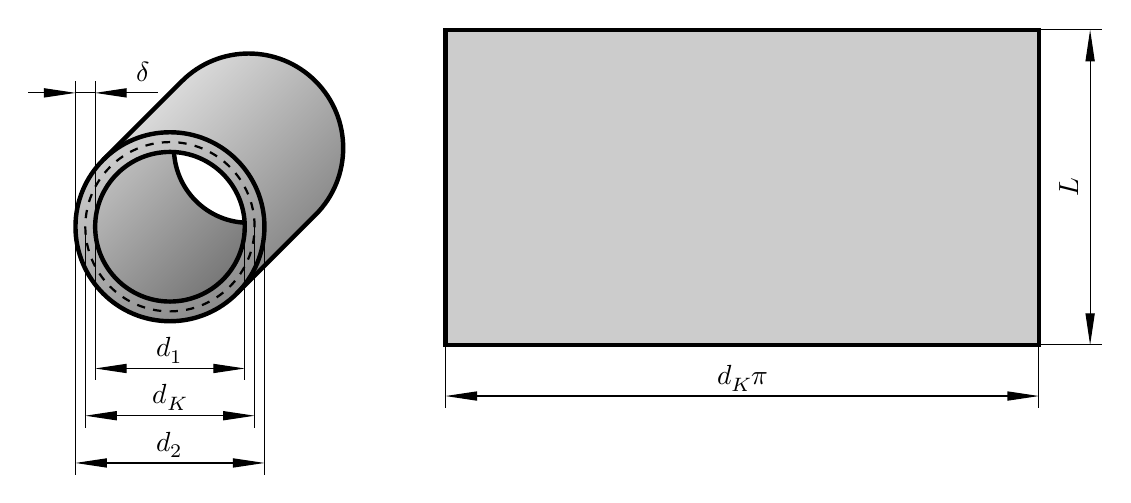
\begin{tikzpicture}
		\pgfmathsetmacro{\DB}{1.9}
		\pgfmathsetmacro{\DK}{2.4}
		
		\shade[shading=axis, bottom color=black!20, top color=black!60, shading angle=-135, even odd rule] (0,0) circle[radius=\DB/2] (1, 1) circle[radius=\DB/2];
		\draw[ultra thick] (1, 1) circle[radius=\DB/2];
		
		\shade[shading=axis, bottom color=black!10, top color=black!50, shading angle=-135] ({-\DK/2/sqrt(2)}, {\DK/2/sqrt(2)}) arc [start angle=135, end angle=-45, radius={\DK/2}] -- ({1+\DK/2/sqrt(2)}, {1-\DK/2/sqrt(2)}) arc [start angle=-45, end angle=135, radius={\DK/2}] -- cycle;
		
		\shade[shading=axis, bottom color=black!20, top color=black!45, shading angle=-150, even odd rule] (0,0) circle[radius=\DK/2] circle[radius=\DB/2];
		
		\draw[ultra thick] ({-\DK/2/sqrt(2)}, {\DK/2/sqrt(2)}) -- ({1-\DK/2/sqrt(2)}, {1+\DK/2/sqrt(2)}) arc [start angle=135, end angle=-45, radius={\DK/2}] -- ({\DK/2/sqrt(2)}, {-\DK/2/sqrt(2)});
		
		\draw[ultra thick] (0, 0) circle[radius=\DB/2];
		\draw[ultra thick] (0, 0) circle[radius=\DK/2];
		\draw[thick, dashed] (0, 0) circle[radius={(\DB+\DK)/4}];
		
		\pgflength[xa=-\DB/2, ya=0, xb=\DB/2, yb=0, ra=\DK/2+0.6]{$d_1$};
		\pgflength[xa={-\DB/4-\DK/4}, ya=0, xb={\DB/4+\DK/4}, yb=0, ra=\DK/2+1.2]{$d_K$};
		\pgflength[xa=-\DK/2, ya=0, xb=\DK/2, yb=0, ra=\DK/2+1.8]{$d_2$};
		
		\pgflength[xa=-\DK/2, ya=0, xb=-\DB/2, yb=0, ra=-\DK/2-0.5, belül=2]{$\delta$};
		
		\draw[ultra thick, fill=black!20] (3.5, -1.5) rectangle ({3.5+\DK*3.14},{2.5});
		\pgflength[xa=3.5, ya=-1.5, xb={3.5+\DK*3.14}, yb=-1.5]{$d_K \pi$};
		\pgflength[xa={3.5+\DK*3.14}, ya=-1.5, xb={3.5+\DK*3.14}, yb=2.5]{$L$};
		
	\end{tikzpicture}
	\caption{Hengeres fal kiterítése és közelítése síkfallal.}
\end{figure}

A hőáramra vonatkozó valós és a közelítő összefüggés:
\begin{equation}
	\dot{Q}_{\textit{valós}} = \dfrac{2 \pi \lambda L}{\ln\frac{d_2}{d_1}} \left(T_1 - T_2\right) 
	\quad \textrm{és} \quad 
	\dot{Q}_{\textit{közelítő}} = \dfrac{2 \lambda}{d_2 - d_1} \dfrac{d_1 + d_2}{2} \pi L\left(T_1 - T_2\right)
\end{equation}

A vizsgálatot a $\varphi = \dfrac{d_2}{d_1} \in \left[1, 3\right]$ intervallumban, 0,5-es lépésekben végezzük el. A vizsgálat az $\varepsilon$ relatív hiba értékének kiszámítását jelenti a $\varphi$ átmérőhányados különböző értékei mellett. A relatív hiba, behelyettesítve a hőáramokat:
\vspace{-2mm}
\begin{equation}
	\varepsilon = \dfrac{\dot{Q}_{\textit{valós}} - \dot{Q}_{\textit{közelítő}}}{\dot{Q}_{\textit{valós}}} = 1 - \dfrac{\dot{Q}_{\textit{közelítő}}}{\dot{Q}_{\textit{valós}}} = 
	1 - \dfrac{
		\dfrac{\bcancel{2} \bcancel{\lambda}}{d_2 - d_1} \dfrac{d_1 + d_2}{2} \bcancel{\pi} \bcancel{L} \cancel{\left(T_1 - T_2\right)}
	}{
		\dfrac{\bcancel{2} \bcancel{\pi} \bcancel{\lambda} \bcancel{L}}{\ln\frac{d_2}{d_1}} \cancel{\left(T_1 - T_2\right)}
	}
\end{equation}

Kifejezve $d_2$-t $\varphi d_1$ alakban:
\begin{equation}
	\varepsilon = 
	1 - \dfrac{d_1 + d_2}{d_2 - d_1} \dfrac{1}{2} \ln\frac{d_2}{d_1} = 
	1 - \dfrac{d_1 + \varphi d_1}{\varphi d_1 - d_1} \dfrac{1}{2} \ln\varphi = 
	1 - \dfrac{1 + \varphi}{\varphi - 1} \dfrac{1}{2} \ln\varphi
\end{equation}

A relatív hiba értékei a vizsgált intervallumban:

\begin{table}[h!]
	\centering
	{\tabulinesep=1.2mm
		\begin{tabu} {|l |[1.5pt] c | c | c | c | c|}
			\hline
			$\varphi$ & 1 & 1,5 & 2 & 2,5 & 3
			\\ \tabucline [1.5pt]{-}
			$\varepsilon\!\left(\varphi\right)$ & 
			$\displaystyle \lim_{\varphi\to 1+} \varepsilon\!\left(\varphi\right) = 0$ &
				0,0134 & 
				0,0382 & 
				0,0645 & 
				0,0897
			\\ \hline
		\end{tabu}
	}
\end{table}

\pagebreak




% 6. fejezet
% ==========
\chapter{Hőterjedés áramló közegben}

% K6/1-es feladat


\section*{K6/1. feladat}
\addcontentsline{toc}{section}{K6/1. feladat}
Egy ellenáramú hőcserélőnél veszteségmentes hőcserét feltételezve a következő adatokat ismerjük: a közegek kezdeti hőmérsékletei $T_{1k} = \SI{140}{\celsius}$ és $T_{2k} = \SI{15}{\celsius}$, a két közeg konvektív vízértéke egyenlő $\dot{w} = \dot{w}_1 = \dot{w}_2 = \SI{58000}{\watt\per\kelvin}$, a hőátszármaztatási tényező $\kappa = \SI{220}{\watt\per\meter\squared\kelvin}$, a teljes hőátadó felület $A_{\ddot{O}} = \SI{100}{\meter\squared}$.

\subsubsection*{a) A véghőmérsékletek meghatározása}
A hőcserélőben történő hőterjedést a következő hőáramokkal jellemezhetjük:
\begin{itemize}
	\setlength\itemsep{0em}
	\item Az \ding{172}-es közeg belépő hőszállításos hőárama $\dot{w}_1 T_{1k}$, a kilépő hőszállításos hőáram $\dot{w}_1 T_{1v}$, a kettő különbsége az \ding{172}-es közeg által \textbf{leadott} $\Delta \dot{Q}_1 = \dot{w}_1 \left(T_{1v} - T_{1k}\right)$; negatív, mert az \ding{172}-es közeg hőmérséklete csökken.
	\item Az átszármaztatott hőáram $\Delta \dot{Q}_{\acute{a}tsz} = \kappa A_{\ddot{O}} \Delta T_{k\ddot{o}z,ln}$, értéke pozitív, a számításánál figyelembe kell venni, hogy a $\dot{w}_1 = \dot{w}_2$ egyenlőség miatt a két közeg közötti hőmérsékletkülönbség állandó $\Delta T = \Delta T_N = \Delta T_K$, és ezzel egyenlő a logaritmikus közepes hőmérsékletkülönbség is.
	
	\begin{equation}
		\dot{w}_1 = \dot{w}_2 \quad \Rightarrow \quad \Delta T_{k\ddot{o}z,ln} = \lim_{\Delta T_N \to \Delta T_K} \dfrac{\Delta T_N - \Delta T_K}{\ln\frac{\Delta T_N}{\Delta T_K}} = \Delta T_N = \Delta T_K = \Delta T
	\end{equation}
	
	A $\Delta T$ hőmérsékletkülönbség felírható a megfelelő vég- és kezdeti hőmérsékletek különbségeként, például $\Delta T = T_{1v} - T_{2k}$.
	
	\item A \ding{173}-es közeg belépő hőszállításos hőárama $\dot{w}_2 T_{2k}$, a kilépő hőszállításos hőáram $\dot{w}_2 T_{2v}$, a kettő különbsége a \ding{173}-es közeg által \textbf{felvett} $\Delta \dot{Q}_2 = \dot{w}_2 \left(T_{2v} - T_{2k}\right)$; pozitív, mert a \ding{173}-es közeg hőmérséklete növekszik.
\end{itemize}

A három hőáram az energiamegmaradás miatt egyenlő, ez alapján a két ismeretlen véghőmérsékletre egy kétismeretlenes egyenletrendszert tudunk felírni (behelyettesítve $\Delta T$-t és a közös $\dot{w}$-t):
\begin{equation}
	-\Delta \dot{Q}_1 = \Delta \dot{Q}_{\acute{a}tsz} = \Delta \dot{Q}_2
	\quad \Rightarrow \quad 
	\left.
		\begin{array}{l}
			I.\: -\dot{w} \left(\highlight{cyan}{T_{1v}} - T_{1k}\right) 
			= 
			\kappa A_{\ddot{O}} \left(\highlight{cyan}{T_{1v}} - T_{2k}\right) \\ \\
			II.\: -\dot{w} \left(\highlight{cyan}{T_{1v}} - T_{1k}\right) 
			= 
			\dot{w} \left(\highlight{orange!75!yellow}{T_{2v}} - T_{2k}\right)
		\end{array}
	\right\rbrace
\end{equation}

Az egyenletrendszer lineáris, a véghőmérsékletek átrendezéssel kifejezhetők:
\begin{equation}
	\highlight{cyan}{T_{1v}} = \frac{\kappa A_{\ddot{O}} T_{2k} + \dot{w} T_{1k}}{\kappa A_{\ddot{O}} + \dot{w}} = \SI{105.625}{\celsius}
\end{equation}
\begin{equation}
	\highlight{orange!75!yellow}{T_{2v}} = T_{2k} + T_{1k} - T_{1v} = \SI{49.375}{\celsius}
\end{equation}

\subsubsection*{b) Mekkora kellene legyen a hőátszármaztatási tényező, hogy a két véghőmérséklet egyenlő legyen?}
A feltétel egyenlet alakban $T_{1v} = T_{2v}$. Mivel a konvektív vízértékek továbbra is egyenlők, a $T\left(A\right)$ hőmérséklet-hely függvények lineárisak és azonos meredekségűek, ezért a két véghőmérséklet úgy lehet egyenlő, ha a kezdeti hőmérsékletek átlagával is egyenlők:
\begin{equation}
	T_{1v} = T_{2v} = \dfrac{T_{1k} + T_{2k}}{2} = \SI{77.5}{\celsius}
\end{equation}

A módosított $\kappa^*$ hőátszármaztatási tényező az átszármaztatott és az egyik szállításos hőáram egyenlőségéből kifejezhető:
\begin{equation}
	-\Delta \dot{Q}_1 = \Delta \dot{Q}_{\acute{a}tsz}
	\quad \Rightarrow \quad 
	-\dot{w} \left(T_{1v} - T_{1k}\right) 
	= 
	\highlight{green!75!black}{\kappa^*} A_{\ddot{O}} \left(T_{1v} - T_{2k}\right)
\end{equation}

Kifejezve a hőátszármaztatási tényező:
\begin{equation}
	\highlight{green!75!black}{\kappa^*} 
	= 
	\dfrac{\dot{w} \left(T_{1k} - T_{1v}\right)}{A_{\ddot{O}} \left(T_{1v} - T_{2k}\right)} 
	= 
	\dfrac{\dot{w} \Delta T}{A_{\ddot{O}} \Delta T} 
	= 
	\dfrac{\dot{w}}{A_{\ddot{O}}} = \SI{580}{\watt\per\meter\squared\kelvin}
\end{equation}

\subsubsection*{c) A léptékhelyes hőmérséklet-hely függvények}
Hőcserélőknél a hőmérséklet-hely függvény a $T\!\left(A\right)$ függvény, amit közegenként különböző, és a helyet az $A$ érintett hőátadó felület jelenti. Az a) és b) részben a konvektív vízértékek egyenlők, ezért lineárisak a $T\!\left(A\right)$ függvények.

\begin{figure}[h]
	\begin{subfigure}[b]{0.48\textwidth} 
		\centering
		\begin{tikzpicture}
			\pgfmathsetmacro{\L}{4}
			\pgfmathsetmacro{\AÖ}{5}
			
			\pgfmathsetmacro{\kelvin}{34}
			\pgfmathsetmacro{\TAK}{140/\kelvin}
			\pgfmathsetmacro{\TAV}{105.6/\kelvin}
			\pgfmathsetmacro{\TBK}{15/\kelvin}
			\pgfmathsetmacro{\TBV}{49.4/\kelvin}
			
			% Tengelyek
			\draw[->] (0,-1) -- (0,\L+1) node[anchor=north east]{$T$};
			\draw[->] (-1.25,0) -- (\AÖ+1,0) node[anchor=base east, shift={(0,-0.5)}]{$A$};
			
			% Az összes felület
			\draw[gray, dashed] (\AÖ,0) -- (\AÖ,\L+0.5);
			\draw (\AÖ,-0.1) -- (\AÖ,0.1);
			\node[anchor=base, shift={(0,-0.5)}] at (\AÖ,0) {$A_{\ddot{O}}$};
			
			% A két T(A)
			\draw[mid arrow=red, red, ultra thick] (0,\TAK) -- (\AÖ,\TAV);
			\draw[mid arrow=blue, blue, ultra thick] (\AÖ,\TBK) -- (0,\TBV);
			
			% A hőmérséklet értékek
			\draw (-0.1,\TAK) -- (0.1,\TAK);
			\node[anchor=base east] at (0,\TAK) {$T_{1k}$};
			\node[anchor=north east] at (0,\TAK) {$\SI{140}{\celsius}$};
			
			\draw (-0.1,\TBV) -- (0.1,\TBV);
			\node[anchor=base east] at (0,\TBV) {$T_{2v}$};
			
			\draw (-0.1+\AÖ,\TBK) -- (0.1+\AÖ,\TBK);
			\node[anchor=base west] at (\AÖ,\TBK) {$T_{2k}$};
			\node[anchor=north west] at (\AÖ,\TBK) {$\SI{15}{\celsius}$};
			
			\draw (-0.1+\AÖ,\TAV) -- (0.1+\AÖ,\TAV);
			\node[anchor=base west] at (\AÖ,\TAV) {$T_{1v}$};
			
			% A hőmérsékletkülönbség
			\pgflength[xb={\AÖ*0.25}, yb={0.75*\TBV+0.25*\TBK}, xa={\AÖ*0.25}, ya={0.75*\TAK+0.25*\TAV}, alim=0, blim=0, ra=0, ny=0]{$\Delta T$};
			
		\end{tikzpicture}
		\caption{A hőmérséklet-hely függvények az a) esetben.}
	\end{subfigure}
	\begin{subfigure}[b]{0.48\textwidth}
		\centering
		\begin{tikzpicture}
			\pgfmathsetmacro{\L}{4}
			\pgfmathsetmacro{\AÖ}{5}
			
			\pgfmathsetmacro{\kelvin}{34}
			\pgfmathsetmacro{\TAK}{140/\kelvin}
			\pgfmathsetmacro{\TAV}{77.5/\kelvin}
			\pgfmathsetmacro{\TBK}{15/\kelvin}
			\pgfmathsetmacro{\TBV}{77.5/\kelvin}
			
			% Tengelyek
			\draw[->] (0,-1) -- (0,\L+1) node[anchor=north east]{$T$};
			\draw[->] (-1.25,0) -- (\AÖ+1,0) node[anchor=base east, shift={(0,-0.5)}]{$A$};
			
			% Az összes felület
			\draw[gray, dashed] (\AÖ,0) -- (\AÖ,\L+0.5);
			\draw (\AÖ,-0.1) -- (\AÖ,0.1);
			\node[anchor=base, shift={(0,-0.5)}] at (\AÖ,0) {$A_{\ddot{O}}$};
			
			% A két T(A)
			\draw[mid arrow=red, red, ultra thick] (0,\TAK) -- (\AÖ,\TAV);
			\draw[mid arrow=blue, blue, ultra thick] (\AÖ,\TBK) -- (0,\TBV);
			
			% A hőmérséklet értékek
			\draw[black!50, dashed] (0,\TBV) -- (\AÖ,\TAV);
			
			\draw (-0.1,\TAK) -- (0.1,\TAK);
			\node[anchor=base east] at (0,\TAK) {$T_{1k}$};
			\node[anchor=north east] at (0,\TAK) {$\SI{140}{\celsius}$};
			
			\draw (-0.1,\TBV) -- (0.1,\TBV);
			\node[anchor=base east] at (0,\TBV) {$T_{2v}$};
			
			\draw (-0.1+\AÖ,\TBK) -- (0.1+\AÖ,\TBK);
			\node[anchor=base west] at (\AÖ,\TBK) {$T_{2k}$};
			\node[anchor=north west] at (\AÖ,\TBK) {$\SI{15}{\celsius}$};
			
			\draw (-0.1+\AÖ,\TAV) -- (0.1+\AÖ,\TAV);
			\node[anchor=base west] at (\AÖ,\TAV) {$T_{1v}$};
			
			% A hőmérsékletkülönbség
			\pgflength[xb={\AÖ*0.25}, yb={0.75*\TBV+0.25*\TBK}, xa={\AÖ*0.25}, ya={0.75*\TAK+0.25*\TAV}, alim=0, blim=0, ra=0, ny=0]{$\Delta T$};
			
		\end{tikzpicture}
		\caption{A hőmérséklet-hely függvények a b) esetben.}
	\end{subfigure}
\end{figure}
 
A kézzel történő feladatmegoldást gyakran lehet az ábrák közelítő felrajzolásával kezdeni, azonban az görbék jelleghelyes rajzolása általában csak a számítások elvégzése után lehetséges.

\pagebreak


% K6/2-es feladat

% K6/3-as feladat

% K6/4-es feladat


\section*{K6/4. feladat}
\addcontentsline{toc}{section}{K6/4. feladat}
Határozza meg, hogy \textbf{száraz telített vízgőzből} mennyi csapódik le óránként egy $d = \SI{40}{\milli\meter}$ átmérőjű, $L = \SI{1}{\meter}$ magas, függőleges cső külső falára $p = \SI{1.01}{\bar}$ gőznyomás esetén, ha a csőfelület középhőmérséklete $T_F = \SI{60}{\celsius}$! A $p$ nyomáshoz tartozó forráspont $T_S = \SI{100}{\celsius}$.

A víz anyagjellemzői a közepes $T_K=\frac{T_S + T_F}{2}$ hőmérsékleten: a párolgáshő $r = \SI{2257.3}{\kilo\joule\per\kilogram}$, a sűrűség $\varrho_{80} = \SI{971.6}{\kilogram\per\meter\cubed}$, a hővezetési tényező $\lambda_{80} = \SI{0.67}{\watt\per\meter\kelvin}$, a dinamikai viszkozitás $\eta_{80} = \SI{351e-6}{\kilogram\per\meter\second}$.

\vspace{2mm}

Nusselt folyadékréteg elmélete szerint a gőz és a lecsapódó folyadékréteg által befolyt csőfal közötti hőátadási tényező az alábbi alakban számolható, ha a folyadék áramlása réteges/lamináris:
\vspace{-2mm}
\begin{equation}
	\alpha = c \left(\dfrac{r \varrho^2 \lambda^3 g}{\eta H \Delta T}\right)^{\tfrac{1}{4}}
\end{equation}

A $c$ értéke, illetve a $H$ jelentése a cső elhelyezkedésétől függ: függőleges fal vagy cső esetén $c_1 = \SI{0,943}{}$, és $H = L$ (az $L$ a magasság vagy függőleges hossz), vízszintes cső esetén $c_2 = \SI{0,726}{}$, és $H = d$ (a $d$ a külső átmérő).

\subsubsection*{a) Függőleges cső vizsgálata}
A gőz lecsapódása során a rejtett hőt adja le átadással a csőnek. Ezt a két hőáram egyenlőségével írhatjuk le, azaz $\dot{Q}_{\textit{rejtett}} = \dot{Q}_{\textit{átadás}}$. Kifejtve a két hőáram:
\begin{equation}
	\dot{Q}_{\textit{rejtett}} = \dot{m}r \quad \textrm{és} \quad \dot{Q}_{\textit{átadás}} = \alpha A \left(T_S - T_F\right) = \alpha d \pi L \left(T_S - T_F\right)
\end{equation}

A hőátadási tényező függőleges csőnél:
\vspace{-2mm}
\begin{equation}
	\alpha_{\textit{függőleges}} = \SI{0.943}{} \left(\dfrac{r \varrho_{80}^2 \lambda_{80}^3 g}{\eta_{80} L \left(T_S - T_F\right)}\right)^{\tfrac{1}{4}} = \SI{4.338}{\watt\per\meter\squared\kelvin}
\end{equation}

A lecsapódás tömegárama a függőleges helyzetű csövön:
\begin{equation}
	\dot{m}_{\textit{függőleges}} = \dfrac{\alpha_{\textit{függőleges}} d \pi L \left(T_S - T_F\right)}{r} = \SI{9.65e-3}{\kilogram\per\second} = \SI{34.775}{\kilogram\per\hour}
\end{equation}


\subsubsection*{b) Vizsgáljuk meg a lecsapódott gőzmennyiséget akkor is, ha a cső vízszintes helyzetű!}
A hőátadási tényező vízszintes csőnél:
\vspace{-2mm}
\begin{equation}
	\alpha_{\textit{vízszintes}} = \SI{0.943}{} \left(\dfrac{r \varrho_{80}^2 \lambda_{80}^3 g}{\eta_{80} L \left(T_S - T_F\right)}\right)^{\tfrac{1}{4}} = \SI{7.468}{\watt\per\meter\squared\kelvin}
\end{equation}

A lecsapódás tömegárama a vízszintes helyzetű csövön:
\begin{equation}
	\dot{m}_{\textit{vízszintes}} = \dfrac{\alpha_{\textit{vízszintes}} d \pi L \left(T_S - T_F\right)}{r} = \SI{16.6e-3}{\kilogram\per\second} = \SI{59.86}{\kilogram\per\hour}
\end{equation}

\subsubsection*{c) A vízszintes vagy a függőleges elrendezést célszerű választani? Mikor nagyobb a hőátadási tényező?}
A kérdés arra vonatkozik, hogy a $d$ és az $L$ viszonya alapján melyik elrendezést célszerű választani. A feladatot az alábbi egyenlőtlenség alakban célszerű megfogalmazni:
\begin{equation}
	\alpha_{\textit{függőleges}} < \alpha_{\textit{vízszintes}} 
	\quad \Rightarrow \quad 
	c_1 \left(\dfrac{\bcancel{r \varrho^2 \lambda^3 g}}{\cancel{\eta} L \cancel{\Delta T}}\right)^{\tfrac{1}{4}} 
	< 
	c_2 \left(\dfrac{\bcancel{r \varrho^2 \lambda^3 g}}{\cancel{\eta} d \cancel{\Delta T}}\right)^{\tfrac{1}{4}} 
	\quad \Rightarrow \quad 
	\dfrac{c_1^4}{c_2^4} d < L
\end{equation}

Azaz, ha $\SI{2.846}{} d < L$, akkor $\alpha_{\textit{függőleges}} < \alpha_{\textit{vízszintes}}$.

\pagebreak



% 7. fejezet
% ==========
\chapter{Hőcserélők, hőszigetelés}

% K7/1-es feladat

\section*{K7/1. feladat}
\addcontentsline{toc}{section}{K7/1. feladat}

\begin{tabular}{ | p{2cm} | p{14cm} | } 
	\hline
	Név & Szalay István \\ 
	\hline
	Szak & \\ 
	\hline
	Félév & 2019/2020 II. (tavaszi) félév \\ 
	\hline
\end{tabular}
\vspace{0.5cm}

\noindent Egy $A_{\ddot{O}} = \SI{15}{\meter\squared}$ hőátadó felületű csőköteges hőcserélőben $\dot{m}_a = \SI{820}{\kilogram\per\hour}$ tömegáramú cseppfolyós ammóniát kell vízzel lehűtenünk. Az ammónia belépési hőmérséklete $T_{ak} = \SI{25}{\celsius}$, a rendelkezésre álló hűtővíz hőmérséklete $T_{vk} = \SI{12}{\celsius}$.

Ha az ellenáramú hőcserélőn $\dot{m}_v = \SI{1130}{\kilogram\per\hour}$ tömegáramú vizet áramoltatunk keresztül és a hőátszármaztatási tényező $\kappa = \SI{160}{\watt\per\meter\squared\kelvin}$, akkor mekkorák lesznek a kilépési hőmérsékletek?

A víz fajhője $c_v = \SI{4.18}{\kilo\joule\per\kilogram\kelvin}$, az ammónia fajhője $c_a = \SI{4.6}{\kilo\joule\per\kilogram\kelvin}$.

\subsubsection*{a) A hőcserét leíró egyenletek}
Az ammónia a hűtött közeg, ezért ez lesz az \ding{172}-es közeg, a víz pedig a \ding{173}-es. A meghatározandó ismeretlenek a $T_{av}$ és $T_{vv}$ véghőmérsékletek, emiatt két független egyenletet kell felírnunk. A hőcserélőben a leadott, az átszármaztatott és a felvett hőáram az energiamegmaradás miatt egyenlő. A leadott és a felvett hőáram egyenlőségéből a véghőmérsékletekre lineáris egyenletet kapunk, az átszármaztatott hőáram viszont csak akkor ad lineáris egyenletet, ha a konvektív vízértékek egyenlők. 
A konvektív vízértékek:
\begin{equation}
	\dot{w}_a = \dot{m}_a c_a = \SI{1047}{\watt\per\kelvin} 
	\quad \textrm{és} \quad 
	\dot{w}_v = \dot{m}_v c_v = \SI{1312}{\watt\per\kelvin} 
\end{equation}

Később a számítási eredmények ellenőrzésére lesz használható az a tény, hogy a nagyobb konvektív vízértékű közeg hőmérséklete változik kevesebbet.

A konvektív vízértékek nem egyenlők, emiatt célszerű keresni egy másik egyenletet, ami lineáris. Ez lehet a $\Delta T\!\left(A\right)$ hőmérsékletkkülönbség-hely függvény a teljes $A_{\ddot{O}}$ hőátadó felületre.
\begin{equation}
	\Delta T\!\left(A_{\ddot{O}}\right) = \Delta T_N \mathrm{e}^{-\kappa \overrightarrow{\overleftarrow{m}} A_{\ddot{O}}} = \Delta T_K
\end{equation}

Ennél az egyenletnél a $\Delta T_N$ és a $\Delta T_K$ hőmérsékletkülönbségek helyes felírására kell odafigyelni, mivel ellenáramú hőcserénél a \textbf{nagyobb konvektív vízértékű közeg belépésénél van a kisebb hőmérsékletkülönbség}. Azaz vizsgált esetben $\Delta T_N = T_{ak} - T_{vv}$ az ammónia belépésénél és $\Delta T_K = T_{av} - T_{vk}$ a víz belépésénél.

Ezek alapján a két ismeretlen véghőmérsékletre az alábbi kétismeretlenes egyenletrendszert tudjuk felírni:
\begin{equation}
	\label{equation:K71T}
	\begin{array}{l}
		-\Delta \dot{Q}_a = \Delta \dot{Q}_v
		\\ \\
		\Delta T\!\left(A_{\ddot{O}}\right) = \Delta T_K
	\end{array}
	\quad \Rightarrow \quad
	\left.
	\begin{array}{l}
		I.\: -\dot{w}_a \left(\highlight{cyan}{T_{av}} - T_{ak}\right) 
		= 
		\dot{w}_v \left(\highlight{orange!75!yellow}{T_{vv}} - T_{vk}\right) 
		\\ \\
		II.\: \left(T_{ak} - \highlight{orange!75!yellow}{T_{vv}}\right) \mathrm{e}^{-\kappa \overrightarrow{\overleftarrow{m}} A_{\ddot{O}}} = \highlight{cyan}{T_{av}} - T_{vk}
	\end{array}
	\right\rbrace
\end{equation}

A fenti egyenletrendszer megoldható egyszerű átrendezéssel, azonban mivel gyakran előfordul, kialakult egy mátrixos megoldási módszer is.

Mindkét a módszernél célszerű a (\ref{equation:K71T}) egyenletrendszerbe az alábbi mennyiségeket behelyettesíteni:
\begin{equation}
	\label{equation:K71FE}
	\varphi = \dfrac{\dot{w}_1}{\dot{w}_2} = \dfrac{\dot{w}_a}{\dot{w}_v}
	\quad \textrm{és} \quad 
	\eta = \mathrm{e}^{-\kappa \overrightarrow{\overleftarrow{m}} A_{\ddot{O}}}
\end{equation}

A $\varphi$ a konvektív vízértékek hányadosa, az $\eta$ az exponenciális függvény értéke.

\subsubsection*{b) Megoldás átrendezéssel}
A (\ref{equation:K71T}) egyenletrendszer átrendezéssel megoldható. A (\ref{equation:K71FE}) szerinti behelyettesítéssel rövidebbek az egyenletek.
Az $I.$ egyenlet átrendezése, $\varphi$ és $\eta$ behelyettesítése után:
\begin{equation}
	\label{equation:K71TT}
	\left.
	\begin{array}{l}
		I.\: \varphi \left( T_{ak} - \highlight{cyan}{T_{av}} \right) 
		= 
		\highlight{orange!75!yellow}{T_{vv}} - T_{vk} 
	\\ \\
		II.\: \left(T_{ak} - \highlight{orange!75!yellow}{T_{vv}}\right) \eta = \highlight{cyan}{T_{av}} - T_{vk}
	\end{array}
\right\rbrace
\end{equation}

Fejezzük ki $\highlight{orange!75!yellow}{T_{vv}}$-t az $I.$ egyenletből és helyettesítsük be a $II.$-ba:
\begin{equation}
	\label{equation:K71TVV}
	I.\: \highlight{orange!75!yellow}{T_{vv}} = \varphi T_{ak} + T_{vk} - \varphi \highlight{cyan}{T_{av}} 
\end{equation}

\begin{equation}
	II.\: \highlight{cyan}{T_{av}} + \eta \left(\varphi T_{ak} + T_{vk} - \varphi \highlight{cyan}{T_{av}}\right) = \eta T_{ak} + T_{vk}
\end{equation}

\begin{equation}
	\label{equation:K71TAV}
	II.\: \highlight{cyan}{T_{av}} = \dfrac{
		\eta T_{ak} + T_{vk} - \eta \left(\varphi T_{ak} + T_{vk}\right)
		}{
		1-\eta \varphi
		}
	= 
	\SI{15.32}{\celsius}
\end{equation}

Visszahelyettesítve az $I.$ egyenletbe, megkapjuk a víz véghőmérsékletét:
\begin{equation}
	I.\: \highlight{orange!75!yellow}{T_{vv}} = \varphi T_{ak} + T_{vk} - \SI{15.32}{\celsius} =  \SI{19.72}{\celsius} 
\end{equation}


\subsubsection*{c) Megoldás mátrix alakban}
A (\ref{equation:K71TT}) egyenletrendszer átrendezéses megoldást paraméteresen elvégezve mindkét ismeretlen hőmérsékletre az $\mat{T}_v = c\mat{A}\,\mat{T}_k$ mátrix alakra hozható. A (\ref{equation:K71TAV}) egyenlet jobb oldalát alakítsuk a kezdeti hőmérsékletes lineáris kombinációjává:
\begin{equation}
	\highlight{cyan}{T_{av}} = \dfrac{
		\eta \left( 1 - \varphi \right) T_{ak} + \left( 1 - \eta \right) T_{vk}
	}{
		1-\eta \varphi
	}
	=
	\dfrac{1}{1-\eta \varphi}
	\begin{bmatrix}
		\eta \left( 1 - \varphi \right) && 1 - \eta
	\end{bmatrix}
	\begin{bmatrix}
		T_{ak} \\
		T_{vk}
	\end{bmatrix}
\end{equation}

A $II.$ egyenletből kifejezve $\highlight{cyan}{T_{av}}$ és behelyettesítve az $I.$ egyenletbe:
\begin{equation}
	II.\: \highlight{cyan}{T_{av}} = \left(T_{ak} - \highlight{orange!75!yellow}{T_{vv}}\right) \eta + T_{vk}
\end{equation}
\begin{equation}
	I.\: \varphi \left( T_{ak} - \left(T_{ak} - \highlight{orange!75!yellow}{T_{vv}}\right) \eta + T_{vk} \right) 
	= 
	\highlight{orange!75!yellow}{T_{vv}} - T_{vk} 
\end{equation}
\begin{equation}
	\highlight{orange!75!yellow}{T_{vv}}
	=
	\dfrac{
		\varphi \left( T_{ak} - T_{ak} \eta + T_{vk} \right) + T_{vk}
	}{
		1 - \eta \varphi
	}
\end{equation}

Innen a mátrixos alak:
\begin{equation}
	\highlight{orange!75!yellow}{T_{vv}}
	=
	\dfrac{
		\varphi \left( 1 - \eta \right) T_{ak} + T_{vk} \left( 1 + \varphi \right)
	}{
		1 - \eta \varphi
	}
	=
	\dfrac{1}{1-\eta \varphi}
	\begin{bmatrix}
		\varphi \left( 1 - \eta \right) && 1 + \varphi
	\end{bmatrix}
	\begin{bmatrix}
		T_{ak} \\
		T_{vk}
	\end{bmatrix}
\end{equation}

Összevonva két mátrixos egyenlet:
\begin{equation}
	\label{equation:K71TM}
	\begin{bmatrix}
		\highlight{cyan}{T_{av}} \\
		\highlight{orange!75!yellow}{T_{vv}}
	\end{bmatrix}
	=
	\dfrac{1}{1 - \eta \varphi}
	\begin{bmatrix}
		\eta\left(1-\varphi\right) & 1-\eta \\
		\varphi\left(1-\eta\right) & 1-\varphi
	\end{bmatrix}
	\begin{bmatrix}
		T_{ak} \\
		T_{vk}
	\end{bmatrix}
\end{equation}

Itt a $c$ állandót és az $\mat{A}$ mátrix elemeit kell kiszámolni, és képezni velük a kezdeti hőmérsékletek lineáris kombinációit. 

\subsubsection*{d) A léptékhelyes hőmérséklet-hely függvények}
A véghőmérsékletek megrajzolása után megrajzolhatók a hőmérséklet-hely függvények.

\begin{figure}[h]
	\centering
	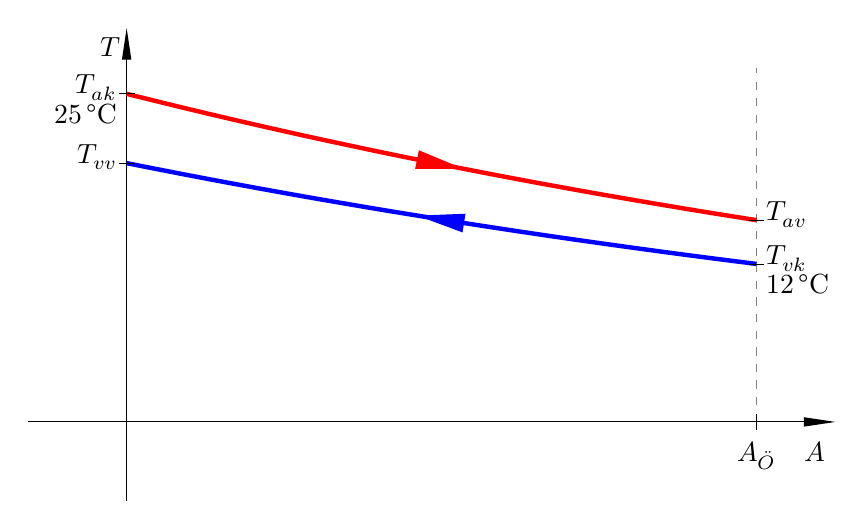
\begin{tikzpicture}
		\pgfmathsetmacro{\L}{4}
		\pgfmathsetmacro{\AÖ}{8}
		
		\pgfmathsetmacro{\kelvin}{6}
		\pgfmathsetmacro{\TAK}{25/\kelvin}
		\pgfmathsetmacro{\TAV}{15.32/\kelvin}
		\pgfmathsetmacro{\TBK}{12/\kelvin}
		\pgfmathsetmacro{\TBV}{19.72/\kelvin}
		
		% Tengelyek
		\draw[->] (0,-1) -- (0,\L+1) node[anchor=north east]{$T$};
		\draw[->] (-1.25,0) -- (\AÖ+1,0) node[anchor=base east, shift={(0,-0.5)}]{$A$};
		
		% Az összes felület
		\draw[gray, dashed] (\AÖ,0) -- (\AÖ,\L+0.5);
		\draw (\AÖ,-0.1) -- (\AÖ,0.1);
		\node[anchor=base, shift={(0,-0.5)}] at (\AÖ,0) {$A_{\ddot{O}}$};
		
		% A két T(A)
		%\draw[red, ultra thick] (0,\TAK) -- (\AÖ,\TAV);
		%\draw[mid arrow=blue, blue, ultra thick] (\AÖ,\TBK) -- (0,\TBV);
		
		\draw[ultra thick, color=red, mid arrow=red, domain=0:\AÖ, smooth, variable=\A] plot (\A, {%
			\TAK - (\TAK-\TBV)/(1047*0.000192738)*(1 - exp(-0.000192738*160*\A*15/\AÖ) )%
			});
		\draw[ultra thick, color=blue, mid arrow=blue, domain=\AÖ:0, smooth, variable=\A] plot (\A, {%
			\TBV - (\TAK-\TBV)/(1312*0.000192738)*(1 - exp(-0.000192738*160*\A*15/\AÖ) )%
			});
		
		% A hőmérséklet értékek
		\draw (-0.1,\TAK) -- (0.1,\TAK);
		\node[anchor=base east] at (0,\TAK) {$T_{ak}$};
		\node[anchor=north east] at (0,\TAK) {$\SI{25}{\celsius}$};
		
		\draw (-0.1,\TBV) -- (0.1,\TBV);
		\node[anchor=base east] at (0,\TBV) {$T_{vv}$};
		
		\draw (-0.1+\AÖ,\TBK) -- (0.1+\AÖ,\TBK);
		\node[anchor=base west] at (\AÖ,\TBK) {$T_{vk}$};
		\node[anchor=north west] at (\AÖ,\TBK) {$\SI{12}{\celsius}$};
		
		\draw (-0.1+\AÖ,\TAV) -- (0.1+\AÖ,\TAV);
		\node[anchor=base west] at (\AÖ,\TAV) {$T_{av}$};
		
		% A hőmérsékletkülönbség
		%\pgflength[xb={\AÖ*0.25}, yb={0.75*\TBV+0.25*\TBK}, xa={\AÖ*0.25}, ya={0.75*\TAK+0.25*\TAV}, alim=0, blim=0, ra=0, ny=0]{$\Delta T$};
		
	\end{tikzpicture}
	\caption{A hőmérséklet-hely függvények.}
\end{figure}

A kézzel történő feladatmegoldást gyakran lehet az ábrák közelítő felrajzolásával kezdeni, azonban az görbék jelleghelyes rajzolása általában csak a számítások elvégzése után lehetséges.

\pagebreak


% K7/2-es feladat


\section*{K7/2. feladat}
\addcontentsline{toc}{section}{K7/2. feladat}
Egy olajipari hűtőnél mérés útján határozzuk meg a hőátszármaztatási tényezőt, a környezeti hatást, és rajzoljuk le axonometrikusan a hőcserélőt!

A hőcserélő 1-4-es (azaz köpenyoldalon 1-szeres, csőoldalon 4-szeres) átfutású, a csőkötegben hűtővíz, a köpenyoldalon benzin  áramlik. Hőszigetelés nincs, a "hőveszteség", a benzinből a környezetbe távozó hő valójában nyereség, ennyivel kevesebb hűtővíz szükséges. A benzin a hűtött közeg, ezért ez lesz az \ding{172}-es közeg, a víz pedig a \ding{173}-es.

A benzin tömegárama $\dot{m}_B = \SI{66000}{\kilogram\per\hour}$, sűrűsége $\varrho_B = \SI{740}{\kilogram\per\meter\squared}$, fajhője $c_B = \SI{2.26}{\kilo\joule\per\kilogram\kelvin}$. A benzin kezdeti hőmérséklete $T_{1k} = \SI{68}{\celsius}$, véghőmérséklete $T_{1v} = \SI{47}{\celsius}$ (a változás $\SI{21}{\celsius}$).

A víz tömegárama $\dot{m}_V = \SI{45400}{\kilogram\per\hour}$, sűrűsége $\varrho_V = \SI{997}{\kilogram\per\meter\squared}$ ($\SI{23}{\celsius}$ hőmérsékletes), fajhője $c_V = \SI{4.179}{\kilo\joule\per\kilogram\kelvin}$. A víz kezdeti hőmérséklete $T_{2k} = \SI{15}{\celsius}$, véghőmérséklete $T_{2v} = \SI{31}{\celsius}$ (a változás $\SI{16}{\celsius}$).

A névleges hőátadó felület $A_{\ddot{O}} = \SI{100}{\meter\squared}$.

\subsubsection*{a) Készítse el a hőcserélő mérési vázlatát és rajzolja meg a hőmérséklet-hely függvényt!}
A mérési vázlat a hőcserélő főbb jellemzőit ábrázolja, nem feltétlenül a térbeli elhelyezkedésük szerint, hanem a lehető legegyszerűbben. A négyszeres köpenyoldali átfutást például elegendő kiterítve, egy-egy csővel jelölni.

\vspace{-5mm}

\begin{figure}[h]
	\centering
	\begin{tikzpicture}[every path/.style={line cap=rect}]
		\pgfmathsetmacro{\D}{3.5}		% A köpeny átmérője
		\pgfmathsetmacro{\L}{8}			% A köpeny hossza
		\pgfmathsetmacro{\p}{0.2}
		
		\pgfmathsetmacro{\NA}{1}		% Csőoldali átfutás (NEM CSINÁLTAM MEG)
		\pgfmathsetmacro{\NB}{4}		% Köpenyoldali átfutás
		\pgfmathsetmacro{\NT}{4}		% Terelőlemez (LEGYEN PÁROS)
		\pgfmathparse{floor(\NT/2)*2}
		\pgfmathsetmacro{\NT}{\pgfmathresult}
		
		\pgfmathsetmacro{\DCS}{0.3}		% Csonkátmérő
		\pgfmathsetmacro{\RS}{\D/\NB}	% Saroksugár
		\pgfmathsetmacro{\RK}{\D/(\NB+1)/2/3}		% Csősugár
		
		\pgfmathsetmacro{\kOldal}{0}	% Köpeny átfolyás [balra(↑←↰)]/jobbra(↱→↑) [0]/1 (mindig felfele)
		
		% Színek
		\colorlet{Hideg}{blue}
		\colorlet{Meleg}{red}
		
		% Fejek
		\fill[Hideg!25] (0,0) -- (-\D/2+\RS,0) arc[start angle=-90, end angle=-180, radius={\RS}] -- (-\D/2, \D-\RS) arc[start angle=180, end angle=90, radius={\RS}] -- (0, \D);
		\draw[-, ultra thick] (-\p, -\p) -- (-\p,0) -- (-\D/2+\RS,0) arc[start angle=-90, end angle=-180, radius={\RS}] -- (-\D/2, \D-\RS)  arc[start angle=180, end angle=90, radius={\RS}] -- (-\p, \D) -- (-\p, \D+\p);
		
		\fill[Hideg!25] (\L, 0) -- (\L+\D/2-\RS,0) arc[start angle=-90, end angle=0, radius={\RS}] -- (\L+\D/2, \D-\RS)  arc[start angle=0, end angle=90, radius={\RS}] -- (\L, \D);
		\draw[-, ultra thick] (\L+\p, -\p) -- (\L+\p,0) -- (\L+\D/2-\RS,0) arc[start angle=-90, end angle=0, radius={\RS}] -- (\L+\D/2, \D-\RS)  arc[start angle=0, end angle=90, radius={\RS}] -- (\L+\p, \D) -- (\L+\p, \D+\p);
		
		% Csőoldali csonkok
		\fill[Hideg!25, xshift={-\D/2*1cm}, yshift={\D/\NB*(1-0.5)*1cm}, rotate=90] ({-\DCS/2}, -\D/4) -- ({-\DCS/2}, 2*\DCS) -- ({\DCS/2}, 2*\DCS) -- ({\DCS/2}, -\D/4);
		\fill[Hideg!25, xshift={-\D/2*1cm}, yshift={\D/\NB*(\NB-0.5)*1cm}, rotate=90] ({-\DCS/2}, -\D/4) -- ({-\DCS/2}, 2*\DCS) -- ({\DCS/2}, 2*\DCS) -- ({\DCS/2}, -\D/4);
		
		\begin{scope}
			% Körülvágás és a globális stílusok összeakadnak
			\tikzset{every path/.style={}}
			\pgfmathsetmacro{\o}{2*\pgflinewidth}
			\clip (-\D cm,\o pt) -- (-\D/2*1cm+\RS*1cm, \o pt) arc[start angle=-90, end angle=-180, radius={\RS*1cm-\o}] -- (-\D/2*1cm + \o, {\D*1cm-\RS*1cm}) arc[start angle=180, end angle=90, radius={\RS*1cm-\o}] -- (-\D cm, {\D*1cm-\o}) -- cycle;
			
			\draw[ultra thick, xshift={-\D/2*1cm}, yshift={\D/\NB*(1-0.5)*1cm}, rotate=90] ({-\DCS/2}, -\D/4) -- ({-\DCS/2}, 2*\DCS) -- ({-\DCS/2 -\p}, 2*\DCS) -- ({\DCS/2 + \p}, 2*\DCS) -- ({\DCS/2}, 2*\DCS) -- ({\DCS/2}, -\D/4);
			\draw[ultra thick, xshift={-\D/2*1cm}, yshift={\D/\NB*(\NB-0.5)*1cm}, rotate=90] ({-\DCS/2}, -\D/4) -- ({-\DCS/2}, 2*\DCS) -- ({-\DCS/2 -\p}, 2*\DCS) -- ({\DCS/2 + \p}, 2*\DCS) -- ({\DCS/2}, 2*\DCS) -- ({\DCS/2}, -\D/4);
		\end{scope}
		
		% Köpeny
		\fill[Meleg!25] (0,0) -- (\L,0) -- (\L, \D) -- (0, \D) -- cycle;
		\draw[-, ultra thick] (0, -\p) -- (0,0) -- (\L,0) -- (\L, -\p) -- (\L, \D+\p) -- (\L, \D) -- (0, \D) -- (0, \D+\p) -- cycle;
		
		% Köpenyoldali terelőlemezek
		\foreach \i in {1,...,\NT}{
			\pgfmathparse{Mod(\i,2)==\kOldal?1:0}
			\ifnum\pgfmathresult>0
				\draw[ultra thick] ({\L/(1+\NT)*\i}, 0) -- ({\L/(1+\NT)*\i}, 2/3*\D);
			\else
				\draw[ultra thick] ({\L/(1+\NT)*\i}, 1/3*\D) -- ({\L/(1+\NT)*\i}, \D);
			\fi
			}
		
		% Köpenyoldali csonkok + FELIRATOK
		\ifnum\kOldal=0
			% balra(↑←↰)
			\pgfmathsetmacro{\dxf}{\L/(1+\NT)/2*1cm}
			\pgfmathsetmacro{\dxa}{\L cm -\L/(1+\NT)/2*1cm}
		\else
			% jobbra(↱→↑)
			\pgfmathsetmacro{\dxf}{(\L-\L/(1+\NT)/2)*1cm}
			\pgfmathsetmacro{\dxa}{\L/(1+\NT)/2 * 1cm}
		\fi
		
		\fill[Meleg!25, xshift=\dxf, yshift=\D cm] ({-\DCS/2}, -\p) -- ({-\DCS/2}, 2*\DCS) -- ({\DCS/2}, 2*\DCS) -- ({\DCS/2}, -\p);
		\draw[ultra thick, xshift=\dxf, yshift=\D cm] ({-\DCS/2}, 0) -- ({-\DCS/2}, 2*\DCS) -- ({-\DCS/2 -\p}, 2*\DCS) -- ({\DCS/2 + \p}, 2*\DCS) -- ({\DCS/2}, 2*\DCS) -- ({\DCS/2}, 0);
		
		\fill[Meleg!25, xshift=\dxa, rotate=180] ({-\DCS/2}, -\p) -- ({-\DCS/2}, 2*\DCS) -- ({\DCS/2}, 2*\DCS) -- ({\DCS/2}, -\p);
		\draw[ultra thick, xshift=\dxa, rotate=180] ({-\DCS/2}, 0) -- ({-\DCS/2}, 2*\DCS) -- ({-\DCS/2 -\p}, 2*\DCS) -- ({\DCS/2 + \p}, 2*\DCS) -- ({\DCS/2}, 2*\DCS) -- ({\DCS/2}, 0);
		
		% Csőkötegfalak
		\draw[-, ultra thick] (-\p/2, -\p) -- (-\p/2, \D+\p);
		\draw[-, ultra thick] (\L+\p/2, -\p) -- (\L+\p/2, \D+\p);
		
		% Csövek
		\foreach \i in {1,...,\NB}{
			\fill[Hideg!25, yshift={\D/\NB*(\i-0.5)*1cm}] (-\p, -\RK) -- (\L+\p, -\RK) -- (\L+\p, \RK) -- (-\p, \RK);
			\draw[ultra thick, yshift={\D/\NB*(\i-0.5)*1cm}] (0, -\RK) -- (\L, -\RK);
			\draw[ultra thick, yshift={\D/\NB*(\i-0.5)*1cm}] (\L, \RK) -- (0, \RK);
			}
		
		% Csőoldali terelőlemezek
		\foreach \i in {2,...,\NB}{
			\pgfmathparse{Mod(\i,2)==0}
			\ifnum\pgfmathresult=1
				\draw[ultra thick, yshift={\D/\NB*(\i-1)*1cm}] (0, 0) -- ({-\D/2}, 0);
			\else
				\draw[ultra thick, yshift={\D/\NB*(\i-1)*1cm}] (\L, 0) -- ({\L+\D/2}, 0);
			\fi
			}
		
		% Csőoldali átfutás
		\draw[->, Hideg, dashed, ultra thick, yshift={\D/\NB/2*1cm}] (-3*\D/8, 0) -- (0, 0);
		\draw[<-, Hideg, dashed, ultra thick, yshift={\D/\NB/2*(2*\NB-1)*1cm}] (-3*\D/8, 0) -- (0, 0);
		\foreach \i in {2,...,\NB}{
			\pgfmathparse{Mod(\i,2)==0}
			\ifnum\pgfmathresult=0
				\draw[<-, Hideg, dashed, ultra thick, yshift={\D/\NB*(\i-1)*1cm}, rotate=180] (0, -\D/\NB/2) -- (\D/10, -\D/\NB/2) arc[radius={\D/\NB/2}, start angle=-90, end angle=90];
			\else
				\draw[->, Hideg, dashed, ultra thick, xshift={\L cm}, yshift={\D/\NB*(\i-1)*1cm}] (\D/10, -\D/\NB/2) arc[radius={\D/\NB/2}, start angle=-90, end angle=90] -- (0, \D/\NB/2);
			\fi
			}
		
		% Köpenyoldali átfutás
		\ifnum\kOldal=1
			\foreach \i in {1,...,\NT}{
				\pgfmathparse{Mod(\i,2)==1}
				\ifnum\pgfmathresult=1
					\draw[<-, Meleg, dashed, ultra thick, xshift={\L/(1+\NT)*\i * 1cm}, yshift={2/3*\D*1cm}] ({\L/(1+\NT)/2}, {-\L/(1+\NT)/2}) -- ({\L/(1+\NT)/2}, 0) arc[radius={\L/(1+\NT)/2}, start angle=0, end angle=180];
				\else
					\draw[->, Meleg, dashed, ultra thick, xshift={\L/(1+\NT)*\i * 1cm}, yshift={1/3*\D*1cm}, rotate=180] ({\L/(1+\NT)/2}, 0) arc[radius={\L/(1+\NT)/2}, start angle=0, end angle=180] -- ({-\L/(1+\NT)/2}, {-\L/(1+\NT)/2});
				\fi
				}
		\else
			\foreach \i in {1,...,\NT}{
				\pgfmathparse{Mod(\i,2)==0}
				\ifnum\pgfmathresult=1
					\draw[->, Meleg, dashed, ultra thick, xshift={\L/(1+\NT)*\i * 1cm}, yshift={2/3*\D*1cm}] ({\L/(1+\NT)/2}, 0) arc[radius={\L/(1+\NT)/2}, start angle=0, end angle=180] -- ({-\L/(1+\NT)/2}, {-\L/(1+\NT)/2});
				\else
					\draw[<-, Meleg, dashed, ultra thick, xshift={\L/(1+\NT)*\i * 1cm}, yshift={1/3*\D*1cm}, rotate=180] ({\L/(1+\NT)/2}, {-\L/(1+\NT)/2}) -- ({\L/(1+\NT)/2}, 0) arc[radius={\L/(1+\NT)/2}, start angle=0, end angle=180];
				\fi
				}
		\fi
		
		% FELIRATOZÁS
		
		% Csőoldal
		\draw[<-,Hideg, ultra thick, xshift={-\D/2*1cm-2*\DCS*1cm-\p*1cm}, yshift={\D/\NB/2*(2*\NB-1)*1cm}] (-3*\D/8, 0) -- (0, 0);
		\node[anchor=south, xshift={-\D/2*1cm-2*\DCS*1cm-\p*1cm}, yshift={\D/\NB/2*(2*\NB-1)*1cm}] at (-3*\D/16, 0) {\ding{173}};
		\node[anchor=north, xshift={-\D/2*1cm-2*\DCS*1cm-\p*1cm}, yshift={\D/\NB/2*(2*\NB-1)*1cm}] at (-3*\D/16, 0) {$T_{2v}$};
		
		\draw[->,Hideg, ultra thick, xshift={-\D/2*1cm-2*\DCS*1cm}, yshift={\D/\NB/2*1cm}] (-3*\D/8, 0) -- (0, 0);
		\node[anchor=south, xshift={-\D/2*1cm-2*\DCS*1cm-\p*1cm}, yshift={\D/\NB/2*1cm}] at (-3*\D/16, 0) {\ding{173}};
		\node[anchor=north, xshift={-\D/2*1cm-2*\DCS*1cm-\p*1cm}, yshift={\D/\NB/2*1cm}] at (-3*\D/16, 0) {$T_{2k}$};
		
		% Köpenyoldal
		% Baloldal fent
		\draw[->, Meleg, ultra thick, xshift=\dxf, yshift={\D cm+2*\DCS cm+\p cm}] (0, 0) -- (0, 1);
		\node[anchor=north west, xshift=\dxf, yshift={\D cm+2*\DCS cm+\p cm+0.5cm}] at (0, 0) {$T_{1v}$};
		\node[anchor=north east, xshift=\dxf, yshift={\D cm+2*\DCS cm+\p cm+0.5cm}] at (0, 0) {\ding{172}};
		
		% Jobboldal lent
		\draw[->, Meleg, ultra thick, xshift=\dxa, yshift={-2*\DCS cm-\p cm - 1cm}] (0, 0) -- (0, 1);
		\node[anchor=north west, xshift=\dxa, yshift={-2*\DCS cm-\p cm - 0.5cm}] at (0, 0) {$T_{1k}$};
		\node[anchor=north east, xshift=\dxa, yshift={-2*\DCS cm-\p cm - 0.5cm}] at (0, 0) {\ding{172}};
		
		% TA HŐMÉRSÉKLET-HELY FÜGGVÉNY
		\pgfmathsetmacro{\L}{4.75}
		\pgfmathsetmacro{\AÖ}{8}
		
		\pgfmathsetmacro{\DY}{-7.5 cm}
		
		\pgfmathsetmacro{\kelvin}{13}
		\pgfmathsetmacro{\TAK}{68/\kelvin}
		\pgfmathsetmacro{\TAV}{47/\kelvin}
		\pgfmathsetmacro{\TBK}{15/\kelvin}
		\pgfmathsetmacro{\TBV}{31/\kelvin}
		
		\begin{scope}
			\tikzset{every path/.style={yshift=\DY}}
			
			% Tengelyek
			\draw[->] (0,-1) -- (0,\L+1.5) node[anchor=north east]{$T$};
			\draw[->] (-1.25,0) -- (\AÖ+1,0) node[anchor=base east, shift={(0,-0.5)}]{$A$};
			
			% Az összes felület
			\draw[gray, dashed] (\AÖ,0) -- (\AÖ,\L+0.5);
			\draw (\AÖ,-0.1) -- (\AÖ,0.1);
			\node[anchor=base, shift={(0,-0.5)}] at (\AÖ,0) {$A_{\ddot{O}}$};
			
			% A hőmérséklet értékek
			\draw[gray, dashed] (0,\TAK) -- (\AÖ+0.5,\TAK);
			\draw (-0.1,\TAK) -- (0.1,\TAK);
			\node[anchor=base east] at (0,\TAK) {$T_{1k}$};
			\node[anchor=north east] at (0,\TAK) {$\SI{68}{\celsius}$};
			
			\draw[gray, dashed] (0,\TAV) -- (\AÖ+0.5,\TAV);
			\draw (-0.1,\TAV) -- (0.1,\TAV);
			\node[anchor=base east] at (0,\TAV) {$T_{1v}$};
			\node[anchor=north east] at (0,\TAV) {$\SI{48}{\celsius}$};
			
			\draw[gray, dashed] (0,\TBK) -- (\AÖ+0.5,\TBK);
			\draw (-0.1,\TBK) -- (0.1,\TBK);
			\node[anchor=base east] at (0,\TBK) {$T_{2k}$};
			\node[anchor=north east] at (0,\TBK) {$\SI{15}{\celsius}$};
			
			\draw[gray, dashed] (0,\TBV) -- (\AÖ+0.5,\TBV);
			\draw (-0.1,\TBV) -- (0.1,\TBV);
			\node[anchor=base east] at (0,\TBV) {$T_{2v}$};
			\node[anchor=north east] at (0,\TBV) {$\SI{31}{\celsius}$};
			
			\pgflength[xb=\AÖ, yb=\TBV, xa=\AÖ, ya=\TAK, ra=-0.65, ny=0]{$\Delta T_N$}
			\pgflength[xa=-\AÖ/8, ya=\TBK, xb=-\AÖ/8, yb=\TAV, ra=-0.65, ny=0]{$\Delta T_K$}
			
		\end{scope}
		
		% A többszörös átfutás
		\foreach \i in {1,...,\NB}{
			\pgfmathparse{Mod(\i,2)==0}
			\pgfmathsetmacro{\j}{2*\AÖ/\NB * floor(\i/2)}
			\ifnum\pgfmathresult=0
				\draw[dashed, ultra thick, color=cyan, mid arrow=cyan, domain=0:\AÖ, smooth, variable=\A, yshift=\DY] plot 
				(\A, {\TBV - (\TAK-\TBV)*3.5*(1 - exp(-0.00133*(\AÖ-(\j + \A/\NB))*100/\AÖ) )});
			\else
				\draw[dashed, ultra thick, color=cyan, mid arrow=cyan, domain=\AÖ:0, smooth, variable=\A, yshift=\DY] plot 
				(\A, {\TBV - (\TAK-\TBV)*3.5*(1 - exp(-0.00133*(\AÖ-(\j - \A/\NB))*100/\AÖ) )});
			\fi
			}
		
		% A két T(A)
		\draw[ultra thick, color=red, mid arrow=red, domain=\AÖ:0, smooth, variable=\A, yshift=\DY] plot (\A, {\TAK - (\TAK-\TBV)/0.213816*(1 - exp(-0.00133*(\AÖ-\A)*100/\AÖ) )});
		\draw[ultra thick, color=blue, mid arrow=blue, domain=0:\AÖ, smooth, variable=\A, yshift=\DY] plot (\A, {\TBV - (\TAK-\TBV)*3.5*(1 - exp(-0.00133*(\AÖ-\A)*100/\AÖ) )});
		
		% FELIRATOK
		\node[draw=cyan, ultra thick, dashed, yshift=\DY] at (\AÖ/4, \TBV+0.5) {valós $T_2\!\left(A\right)$};
		\node[draw=blue, ultra thick, yshift=\DY, text width=2.2cm, align=center] at (3*\AÖ/4, \TBV+0.65) {ellenáramú helyettesítés};
		
		
	\end{tikzpicture}
	\caption{A hőcserélő mérési vázlata és a hőmérséklet-hely függvények.}
	\label{figure:K72A}
\end{figure}

A többszörös csőoldali átfutás miatt a hőcserélő vegyesáramú, de a hőmérséklet-hely függvény helyettesíthető egy ellenáramúval.

%\subsubsection*{b) Rajzolja le a hőcserélő robbantott ábráját!}
%[KÉSŐBB]

\subsubsection*{c) A vegyesáramú hőcserélő átszármaztatott hőárama}
A vegyesáramú hőcserélő átszármaztatott hőáram az alábbi összefüggéssel számolható:
\begin{equation}
	\dot{Q}_{\acute{a}tsz} = \kappa A_{\ddot{O}} \Delta T_{k\ddot{o}z,ln} F_t
\end{equation}
ahol $F_t$ a logaritmikus közepes hőmérsékletkülönbség vegyesáram esetén szükséges helyesbítő tényezője.

\subsubsection*{d) A logaritmikus közepes hőmérsékletkülönbség (LMTD)}
A logaritmikus közepes hőmérsékletkülönbség (LMTD: logarithmic mean temperature difference) számításához szükség van a kisebb és nagyobb hőmérsékletkülönbségre. Ezek leolvasásához a $T_2\!\left(A\right)$ hőmérséklet-hely függvényt a megfelelő ellenáramúval kell helyettesíteni (lásd \hyperref[figure:K72A]{\ref{figure:K72A}. ábra}).
\begin{equation}
	\Delta T_{k\ddot{o}z,ln} 
	= 
	\dfrac{\Delta T_N - \Delta T_K}{\ln\dfrac{\Delta T_N}{\Delta T_K}} 
	= 
	\dfrac{\SI{37}{\celsius} - \SI{33}{\celsius}}{\ln\dfrac{\SI{37}{\celsius}}{\SI{33}{\celsius}}} 
	= 
	\SI{34.44}{\celsius} = \SI{34.44}{\kelvin}
\end{equation}

A logaritmikus közepes hőmérsékletkülönbség egy hőmérsékletkülönbség, ezért Celsius-fokban és kelvinben azonos az értéke.

\subsubsection*{e) Az $F_t$ helyesbítő tényező}
Az $F_t$ leolvasásához ki kell számítani a hőmérsékletviszonyokat jellemző $R$ és $S$ hányadosokat. Az $R$ a meleg és hideg közeg hőmérsékletváltozásának hányadosa:
\begin{equation}
	R = \dfrac{\Delta T_1}{\Delta T_2} = \dfrac{T_{1k} - T_{1v}}{T_{2v} - T_{2k}} = \SI{1.31}{}
\end{equation}

Az $S$ a hidegebb közeg hőmérsékletváltozásának és a legnagyobb hőmérsékletkülönbségnek (általában a belépő hőmérsékletek különbségének) hányadosa:
\begin{equation}
	S = \dfrac{\Delta T_2}{\Delta T_{max}} = \dfrac{T_{2v} - T_{2k}}{T_{1k} - T_{2k}} = \SI{0.3}{}
\end{equation}

Az $F_t$ leolvasható értéke 0,95.

\subsubsection*{f) Az átszármaztatott hőáram és a hőátszármaztatási tényező}
Az átszármaztatott hőáramot a hűtővíz által felvett hőárammal tekinthetjük azonosnak, a benzin által leadott hőáram ennél több, mivel a benzin hőjének egy része a környezetbe távozik.
\begin{equation}
	\dot{Q}_{\acute{a}tsz} = \Delta \dot{Q}_{V} = \dot{m}_V c_V \Delta T_2 = \dot{m}_V c_V \left(T_{2v} - T_{2k}\right) = \SI{843.23}{\kilo\watt}
\end{equation}

Innen a hőátszármaztatási tényező:
\begin{equation}
	\kappa = \dfrac{\dot{Q}_{\acute{a}tsz}}{A_{\ddot{O}} \Delta T_{k\ddot{o}z, ln} F_t} = \SI{257.73}{\watt\per\meter\squared\kelvin}
\end{equation}

\subsubsection*{g) A környezeti hatás}
A "hasznos hőveszteségként" megnyilvánuló környezeti hatást a benzin által leadott és a víz által felvett hőáramok különbségeként tudjuk számolni. A benzin által leadott hőáram:
\begin{equation}
	\Delta \dot{Q}_{B} = \dot{m}_B c_B \Delta T_1 = \dot{m}_B c_B \left(T_{1k} - T_{1v}\right) = \SI{870.1}{\kilo\watt}
\end{equation}

A környezeti hatás:
\begin{equation}
	\Delta \dot{Q}_{B} - \Delta \dot{Q}_{V} = \SI{26.9}{\kilo\watt}
\end{equation}

\pagebreak





\end{document}



